\documentclass{l4proj}
\usepackage{enumitem}
\usepackage{booktabs}

\usepackage[T1]{fontenc}
\usepackage[utf8]{inputenc}
\usepackage{babel}
\usepackage[font=small,labelfont=bf]{caption}

\usepackage{hyperref}
\hypersetup{
    colorlinks=true,
    linkcolor=black,    
    urlcolor=cyan,
    citecolor=black
}

\lstdefinelanguage{JavaScript}{
  % types and declarations
  morekeywords = [1]{break, continue, delete, else, for, function, if, in,
    new, return, typeof, var, void, while, with, try, catch, switch, async, await, const, case, let, class, export, throw, import, null, boolean, number, undefined, Array, Boolean, Date, Math, Number, String, Object, void},
  morekeywords = [2]{eval, parseInt, parseFloat, escape, unescape},
  % values
  morekeywords = [3]{true, false},
  %styles
  keywordstyle = [1]\color{blue}\bfseries,
  sensitive,
  morecomment=[s]{/*}{*/},
  morecomment=[l]//,
  morecomment=[s]{/**}{*/},
  morestring=[b]',
  morestring=[b]",
  morestring=[b]`,
}[keywords, comments, strings]

\lstset{language=JavaScript}

\begin{document}

%==============================================================================
%% METADATA
\title{Virtual Lead: A Competition and Web-Based Smartphone Controller for a Self-Driving Robot}
\author{Lewis Trundle}
\date{March 31, 2023}

\maketitle

%==============================================================================
%% ABSTRACT
\begin{abstract}
    Self-driving robot competitions are a way for enthusiasts and individuals interested in the field of robotics to explore, learn, and develop various solutions that allow a robot to autonomously drive. However, often submissions into these competitions are limited by prohibitive costs and restrictions on self-driving approaches. Furthermore, these competitions have become saturated with repetitive solutions, which fail to explore the possibilities that are encompassed by the term \textit{"self-driving"}. This project develops a self-driving robot competition that is accessible for anyone to enter, promotes collaboration, and allows a range of various approaches to self-driving. To understand whether the competition is feasible for entry, we develop a submission into this competition in the form of a robot controller. We develop this controller to run on a web browser and to allow a robot to be manually controlled via a joystick. Furthermore, we present \textit{Virtual Lead}, a new novel approach to autonomous driving, utilising marker detection and integrating modern smartphone technology. Finally, we conduct a user study, to determine the effectiveness of this controller in navigating competition-style environments.
\end{abstract}

%==============================================================================
\setcounter{page}{2}
\chapter*{Acknowledgements}
I would like to express my thanks and gratitude towards my supervisor Jonathan Grizou, for supporting me throughout this project. Without his guidance, this work would not have been possible. I'd also like to express my appreciation towards my friends and family, who've helped support me throughout the many stressful times during this project.

%==============================================================================

% EDUCATION REUSE CONSENT FORM
\def\consentname {Lewis Trundle}
\def\consentdate {31 March 2023}
\educationalconsent


%==============================================================================
\tableofcontents

%==============================================================================
%% Notes on formatting
%==============================================================================
% The first page, abstract and table of contents are numbered using Roman numerals and are not
% included in the page count. 
%
% From now on pages are numbered
% using Arabic numerals. Therefore, immediately after the first call to \chapter we need the call
% \pagenumbering{arabic} and this should be called once only in the document. 
%
% Do not alter the bibliography style.
%
% The first Chapter should then be on page 1. You are allowed 40 pages for a 40 credit project and 30 pages for a 
% 20 credit report. This includes everything numbered in Arabic numerals (excluding front matter) up
% to but excluding the appendices and bibliography.
%
% You must not alter text size (it is currently 10pt) or alter margins or spacing.
%
%
%==================================================================================================================================
\chapter{Introduction}
% reset page numbering. Don't remove this!
\pagenumbering{arabic} 

\section{Motivation}\label{sec:motivation}
In recent years, the field of autonomous robotics has become increasingly popularised in the entertainment industry, with competitions such as the AWS DeepRacer League\footnote{AWS DeepRacer - \url{https://aws.amazon.com/deepracer/}} bringing in an influx of thousands of viewers and competitors every year. Competitions like these present a way for keen enthusiasts of autonomous robotics to showcase their skills, by solving challenges, and collaborating with others to help improve their community.

However, despite this growing popularity, there is still a lack of affordable and accessible competitions. Many platforms require physical participation and can quite often be costly - requiring expensive robots or services, such as the aforementioned DeepRacer project, which heavily encourages using specialised hardware and software, costing hundreds of dollars. Although to a company this may not seem like much, it can be a massive barrier to those who cannot access these types of resources. With no requirement to make winning solutions public, these factors dissuade collaborativity, and contribute towards the autocratization of autonomous robotic competitions, where large, well-funded companies dominate, leaving no room for small-scale, independent enthusiasts.

Additionally, these competitions should allow a wide-variety of autonomous driving techniques to be utilised. This versatility is essential in allowing participants to learn and share a diverse range of different skills which address the given challenges. However, current competitions have become saturated with the same approaches for self-driving, often restricting participants to one specific approach.

These restrictions limit the opportunities for many to participate in the growing field of autonomous robotics. Their unaffordability dissuades individuals such as students from entering due to its costly nature, and their inaccessibility discourages those from different places around the world. Combined, these factors dampen the development of diverse ideas and hinders collaboration and discussion.

With this in mind, the autonomous robotics community could benefit from a new competition - one which is low-cost, available to anyone to enter, promotes collaboration, and allows a wide variety of diverse approaches. Additionally, new novel ideas for self-driving are needed, which encourage the use of unique, inexpensive technologies and methods.


\section{Project Aim}
Following from Motivation \ref{sec:motivation}, the overall aim of this project is to create such a competition for a self-driving robot and prove its viability by entering a submission into the competition. This submission is a controller, which can control a connected robot. The controller should be eligible for submission into the competition and its development will help inform future necessary changed needed for the competition. Outlined below are the specific aims for the competition and controller. 

\subsection{The Competition}\label{sec:comp-aims}
The competition should serve as a platform where developers can showcase their knowledge and expertise in the field of autonomous robotics and compete against others to win the competition. 
\\
\subsubsection{Affordable} \hfill \\
The competition should be affordable to participate in, and should promote the development of low-cost robotics. By doing so, a wider range of those from different backgrounds and socio-economic groups can participate, giving them an opportunity to get more involved with autonomous robots.

\subsubsection{Accessible} \hfill \\
The competition should be available to enter for anyone around the globe, and should not require physical in-person participation, to make sure that those who cannot travel from different areas and countries are not excluded. Additionally, it should not require any additional experience in robotics and should be available for anyone to enter.

\subsubsection{Collaborative} \hfill \\
The competition should unify people from different parts of the world by promoting the collaboration of ideas. It should serve as a platform where people can share their projects and help educate those trying to get into the field by fostering positive relationships between entrants. 

\subsubsection{Versatile} \hfill \\
The competition should allow for a diverse variation among different techniques used for driving autonomously. It should allow for traditional techniques such as colour-detection, line-detection, and object-detection, but should also encourage participants to implement unique, novel approaches.


\subsection{The Controller}\label{sec:controller-aims}
The entry for this competition should challenge participants to design and implement a controller for a robot. This controller should achieve the following aims.
\\
\subsubsection{Promote Affordable Solutions} \hfill \\
The controller should utilise common available resources in order to remain affordable for an individual who may wish to enter the competition.

\subsubsection{Be Accessible to Use} \hfill \\
The controller should be easily accessible to use, requiring no specific requirements, such as expensive hardware, or installation of any software.

\subsubsection{Provide Precise and Responsive Manual Control} \hfill \\
The controller should allow for precise and accurate manual control over the robots movements. Additionally, this should have a responsive design - being able to be used seamlessly by a user.

\subsubsection{Present a Novel Self-Driving Approach} \hfill \\
The controller should present a novel approach to self-driving - incorporating innovative techniques which are not commonly seen in self-driving competitions. By showcasing these features, the possibilities of new, unique technologies can be demonstrated to encourage a wider variety of self-driving methods to be used in the future.


%==================================================================================================================================
\chapter{Background}
This chapter will discuss related research for this project, by first investigating pre-existing robotic competitions and identifying areas on which to improve upon. The chapter will then examine technologies used for communicating with robots, then will finally discuss various devices and methods used to control a robot.

\section{Existing Competitions}
\subsection{Amazon DeepRacer}\label{sec:deepracer}
Announced at the Amazon Web Services re:Invent conference \citep{DeepracerAnnounced}, the Amazon DeepRacer project provides a platform for users to learn various machine learning techniques and get started with reinforcement learning (RL), by implementing a self-driving vehicle \citep{balaji2020deepracer}.

\subsubsection{Affordability} \hfill \\
A key component of the DeepRacer project, is the autonomous 1/18th scale race car, seen in Figure \ref{fig:deepcar}. Equipped with multiple cameras, an RL model can be uploaded onto the car to control the throttle and steering, so that it may navigate around a real physical track. The car is available to buy from Amazon with the current price of \$399 for the basic model\footnote{DeepRacer Car Pricing - \url{https://www.amazon.com/AWS-DeepRacer-Fully-autonomous-developers/dp/B07JMHRKQG}} - £325 according to current USD to GBP exchange rates \citep{exchangerates}. This can be upgraded to the 'Evo' model by buying a sensor kit for an additional \$249 (£203), or buying the whole Evo car for \$598 (£487). However, this car is not currently available to buy in the UK.

In addition to the car, DeepRacers' Simulator console can be used to create, train, and evaluate an RL model. The free AWS tier gives users enough time to train and evaluate their first model. However, for their model to hold up to competition standard, developers would need to pay for additional training and evaluation time - costing \$3.50 (£2.80) per hour\footnote{DeepRacer Simulator Pricing - \url{https://aws.amazon.com/deepracer/pricing}}.

From this, we see that the DeepRacer project lacks many affordable options. The cost of the car and the cost needed to fully train a model can lead to those from poorer economic backgrounds being able to compete. DeepRacer does support a separate league for students\footnote{DeepRacer Student League - \url{https://aws.amazon.com/deepracer/student/}}, which provides a more affordable option. However, this still is only available to students.

\subsubsection{Accessibility} \hfill \\
These models can eventually be put to the test in the DeepRacer League - a competition boasting multiple rounds, each having different rules and challenges. With the competition hosting a mixture of rounds both physically and virtually - the virtual rounds encourages developers from all around the world to enter, making it accessible to those in other countries. While the physical rounds encourages these developers to meet in-person and collaborate on new ideas relating to the competition. Additionally, AWS even allows communities to host their own local leagues.

\subsubsection{Collaborativity and Versatility} \hfill \\
Examples of community ideas can be seen via DeepRacers community projects. This highlights projects made by members of the community, such as the \textit{'Follow the Leader'} project, which allows the DeepRacer car to identify and follow an object \citep{DeepracerFollowTheLeader}, and the \textit{'Off Road'} project which allows the car to follow a waypoint marked by a series of QR codes \citep{DeepracerOffRoad}.

\begin{figure}[!h]
    \centering
    \begin{subfigure}[b]{0.44\textwidth}
        \includegraphics[width=\textwidth]{images/DeepRacer.png}
        \caption{AWS DeepRacer Car. Available for \$399 (£325).}
        \label{fig:deepcar}
    \end{subfigure}
    \quad
    \begin{subfigure}[b]{0.44\textwidth}
        \includegraphics[width=\textwidth]{images/piborg.jpg}
        \caption{PiBorg MonsterBorg Robot. Available for £210.}
        \label{fig:piborg-car}
    \end{subfigure}   
    \caption{Robot vehicles needed for the self-driving robot competitions. \subref{fig:deepcar} shows the AWS DeepRacer Car, needed for the AWS DeepRacer League. \subref{fig:piborg-car} shows the PiBorg MonsterBorg robot, needed for the Formula Pi competition. The robot cars cost \$399 (£325) and £210 respectively.
    }\label{fig:robot-cars}
\end{figure}

\subsection{Formula Pi}\label{sec:formulaPi}
Formula Pi\footnote{Formula Pi - \url{https://www.formulapi.com/}} hosted by PiBorg\footnote{PiBorg - \url{https://www.piborg.org/}}, is a small autonomous robot competition, involving programming small Raspberry Pi powered robots to navigate a race-track. The competition stretches over nine rounds and a pair of finals, where contestants race their robot against each other on the PiBorg Circuit - a 22m long race-track divided into six colour-coded lanes.

\subsubsection{Affordability} \hfill \\
Formula Pi is not entirely affordable. Before entering the competition, contestants must first purchase their robot kit\footnote{MosterBorg kit - \url{https://www.piborg.org/robots-1/monsterborg}} from PiBorg (shown in Figure \ref{fig:piborg-car}), which currently costs £210. This kit comes with all the necessary components to build the autonomous robot; however, additional costs may be needed for those wanting to customise and improve their vehicle.

\subsubsection{Accessibility} \hfill \\
The competition is widely accessible, with Formula Pi encouraging people from all over the world to enter, regardless of location. This accessibility is accommodated by hosting the competition virtually - making participants submit their code for use. Additionally, the MonsterBorg is available to buy in the UK - unlike the AWS DeepRacer Car.

\subsubsection{Collaborativity} \hfill \\
Although Formula Pi does not facilitate any physical collaboration, it does encourage participants to work together to create novel solutions. This helps to establish a community for the competition. Furthermore, the code of the winner is made open-source, and developers are encouraged to view and modify it, so that the following year's entries may be improved.

\subsubsection{Versatility} \hfill \\
In terms of versatility, Formula Pi supports a wide range of self-driving techniques. The PiBorg Circuit allows for robots to use line-detection to follow a lane around the track. The various colours of the track facilitates the use of colour-detection, to help keep the robot restricted to a singular coloured lane. Additionally, since multiple robots can be raced at once, participants are encouraged to implement object-avoidance to avoid other contestants' robots.


\section{Communication Technology}\label{sec:communication-tech}
\subsection{Web Bluetooth}\label{sec:bluetooth-background}
Introduced in 2015 as a proposed standard for web browsers, the Web Bluetooth API\footnote{Web Bluetooth API - \url{https://developer.mozilla.org/en-US/docs/Web/API/Web_Bluetooth_API}} establishes a wireless connection between a web application and a Bluetooth enabled device. This connection allows Bluetooth devices (such as a robot) to be controlled using JavaScript running from a web browser (such as on a mobile device). This provides a simplified approach, where communication can occur seamlessly, removing the need for installation of native applications to enable Bluetooth communication.

A key benefit of Web Bluetooth is its multi-browser compatibility, with popular web-browsers such as Google Chrome and Microsoft Edge, both supporting the full functionality of Web Bluetooth. It also provides additional benefits such as low energy consumption compared to Wi-Fi and support for both Bluetooth Low Energy (BLE) and Bluetooth Classic protocols.

Unfortunately, a fundamental drawback is that Web Bluetooth is not yet supported on iOS devices \citep{webbluetooth}. Workarounds to this do exist however, for example, WebBLE\footnote{WebBLE - \url{https://webble.com/}}, a third-party app which acts as a Bluetooth client, can allow an iOS device to connect to Bluetooth Low Energy devices, from a web-page. However, this can be considered not an effective solution, due to the \$1.99 (£1.60) pricing of the app and its incompatibility with macOS.

\subsection{UART}\label{sec:uart-background}
Facilitated by Web Bluetooth, the UART (Universal Asynchronous Receiver/Transmitter) protocol is used for serial transmission of data \citep{pena2020uart}. Utilised by Espruino devices and commonly integrated in microcontrollers, UART provides a way of asynchronously communicating between devices. This means there is no clock signal which synchronises data transmission. Instead, start and stop bits mark the beginning and end of data packets being transferred.

UART.js is a JavaScript library which provides a simple interface for communicating with devices and sending data over a serial port \citep{uartjs}. The library is designed to work with Web Bluetooth running from a web-page served over HTTPS, and can receive and write data from connected devices. This functionality can be utilised for important purposes, such as reading sensor data, or controlling actuators.

\section{Espruino Devices in Robotics}
\subsection{Zumo Robot}\label{sec:zumo-robot-background}
A popular robot for Mino Sumo competitions (competitions where robots must be less than 10cm x 10cm) is the Zumo Robot for Arduino\footnote{Zumo Robot for Arduino - \url{https://www.pololu.com/category/169/zumo-robot-for-arduino}}. The robot is composed of a Zumo Chassis\footnote{Zumo Chassis - \url{https://www.pololu.com/product/1418}} - a small tracked platform for mounting circuit components - and a Zumo Shield\footnote{Zumo Shield - \url{https://www.pololu.com/product/2508}} - an electronics board which provides control over functionality such as the motors, gyroscope, and IR receiver.

In addition to the hardware components, a microcontroller is needed in order to manage the various functionalities of the Zumo Shield. Arduino boards\footnote{Arduino boards - \url{https://store.arduino.cc/collections/boards}} are commonly used with Zumo robots. These need to be soldered onto the Zumo Shield to access its control pins. Arduino has a vast library of pre-written code, and the microcontrollers are open-source, meaning they can be easily modified. This allows developers to program the robot to perform a diverse array of tasks. 

The Zumo Robot (without the controller) can currently be bought for \$109 (£89). However, a diverse range of components can also be bought and interchanged with parts of the robot, allowing more experienced developers to build a robot suiting their specific needs. Buying these components individually typically results in a higher price, as seen in Table \ref{tab:zumo-robot-components}.

With its versatility and ability to intermix various components, Zumo Robots act as a popular platform for simple hobbyists and enthusiasts to explore robotics and embedded programming. With a moderate initial investment, anyone can get started building their own robot. However, for more extensive customisability, the total cost of buying individual components can eventually add up.

\begin{table}[h!]
\centering
\caption{Cost breakdown of standard components of the Zumo Robot for Arduino. Costs have been converted to GBP using current USD to GBP exchange rates \citep{exchangerates}.}
\label{tab:zumo-robot-components}
\begin{tabular}{|l|l|l|}
\hline
Component & Price (\$) & Price (£) \\ \hline
Zumo Chassis Kit & 19.95 & 16.20 \\ \hline
Zumo Shield for Arduino v1.3 & 34.95 & 28.50\\ \hline
Zumo Reflectance Sensor & 14.95 & 12.20 \\ \hline
Micro Metal Gearmotor (x2) & $\sim$46 & $\sim$37.40 \\ \hline
AA Batteries (x4) & $\sim$3 & $\sim$2.40 \\ \hline
\textbf{Total} & \textbf{118.85} & \textbf{96.70} \\ \hline
\end{tabular}
\end{table}

\subsection{Espruino Pixl.js}\label{sec:pixl-background}
The Espruino Pixl.js\footnote{Espruino Pixl.js - \url{http://www.espruino.com/Pixl.js}} (seen in Figure \ref{fig:pixljs}) is a small programmable Bluetooth device, which comes with Espruino pre-installed - an open-source JavaScript interpreter for microcontrollers. Available for £36, this device comes equipped with an LCD display and a vast variety of sensors for developers to use to their liking. 

JavaScript code can be uploaded to the Pixl.js to control its input and output pins (shown in Figure \ref{fig:pixljs-pinout}). These pins and JavaScript interpreter allow the Pixl.js to integrate with a vast array of Arduino Shields - making it capable of acting as a microcontroller for Zumo robots. With its Bluetooth capabilities, the Pixl.js can receive instructions from the web, via Web Bluetooth, and activate the relevant functionality on the robot - making it ideal to use for a web-based robot controller.

\begin{figure}[h!]
    \centering
    \begin{minipage}[b]{0.43\textwidth}
        \includegraphics[width=\textwidth]{images/pixljs.jpeg}
        \caption{The Espruino Pixl.js device.}
        \label{fig:pixljs}
    \end{minipage}
    \begin{minipage}[b]{0.50\textwidth}
        \includegraphics[width=\textwidth]{images/pixljs-pinout.png}
        \caption{Pin layout for the Pixl.js.}
        \label{fig:pixljs-pinout}
    \end{minipage}
\end{figure}

\section{Integrating Smartphones in Robotics}\label{sec:smartphone-background}
In recent years, modern smartphones have become increasingly powerful, coming equipped with powerful sensors, processors, and cameras. Their computational power has been consistently increasing, which has meant we’ve seen an increase in their usage in modern robotics. Smartphones now have the capability to control vastly complex systems, such as \citet{comma}, which is capable of providing semi-autonomous driving for a vehicle, all from the power of a smartphone device. 

These features can be dependent on the chosen operating system. The two most prevalent modern smartphone operating systems are Google’s Android and Apple’s iOS - both dominate the market, controlling a 72.3\% and 27.1\% worldwide market share respectively \citep{osmarketshare}. However as outlined in the following sections, certain functionality is only available on certain devices and browsers, specific to an operating system. Explored below are factors which should be considered when integrating a smartphone device into a robot, and their limitations given a specific OS, device, or browser.

\subsection{Computational Power}
One of the first examples showcasing the possibilities of a smartphone controlled robot, was by \citet{oros2013smartphone}, who detailed the development of The Android Car - a low-cost robot powered by an Android phone. Described as a \textit{“do-it-yourself (DIY) smartphone based robotic platform”}, the robot was built using common components and open-source libraries, available to simple hobbyists and enthusiasts, and costing only \$350 (£285) (not including the phone). The final product was able to perform colour-tracking and object-avoidance, allowing it to showcase a degree of autonomous driving - showing how expensive, state-of-the-art technology is not essential in being able to create an effective self-driving robot.

Additionally, this paper highlighted the computational power and versatility of the Android smartphone, by showing how it can act as an onboard computer, controlling the behaviour of the robot via a neural network running on the phone. This is an aspect which is continued in later studies, such as one by \citet{7754547}, which used an Android phone to control a Raspberry Pi powered robot. However, this robot differs from The Android Car, in the fact that the smartphone is not attached to the robot. With the Android Car, the phone was attached to the robot, allowing it to take advantage of the available sensors on the phone, such as the camera, and GPS. In this study however, the smartphone is used similar to a physical controller - controlling the robot from nearby.

\subsection{Communication Methods}
Within both of the two aforementioned studies, Wi-Fi is used as the primary method of communication between the smartphone and some other external device. Wi-Fi does have its advantages compared to other communication methods, such as much faster data-transmission rates \citep{hassan2012review}. However, Bluetooth has become an increasingly more common choice as a communication method in smartphone controlled robotics.

The idea of using Bluetooth communication in robotics was explored in the early 2000’s, by \citet{fai2002bluetooth}, who studied how a Bluetooth enabled robot can communicate with a PC device. This proved the viability of Bluetooth as a reliable method of sending instructions between a robot and another device in real-time. This work was continued in 2010 by \citet{nasereddin2010smartphone}, where a smartphone used Bluetooth to communicate with a robot to calculate the shortest path between the robots current position and a position selected by a user. In this experiment, the smartphone received location data from the robots onboard GPS, and was able to effectively process this information into relevant movement instructions for the robot - proving the effectiveness of using Bluetooth as a reliable mechanism to control robotic hardware.

\subsection{OpenBot} \label{sec:openbot}
One of the most recent studies highlighting the use of smartphones in robotics is OpenBot\footnote{OpenBot - \url{https://www.openbot.org/}}, by \citet{muller2021openbot}. Similar to the Android Car, OpenBot leverages the computational power and available sensors of an Android smartphone, by attaching it to the robot and processing data from the camera and other sensors directly on the phone (as seen in Figure \ref{fig:openbot}). This in turn communicates with an Arduino board attached to the robot via serial communication - providing the low-level interface to the vehicle. This is used in conjunction with a Bluetooth connected physical controller, which can provide high-level manual control for attributes such as the steering angle and throttle.

OpenBot utilises a variety of self-driving methods in order to perform complex tasks. For example, computer vision from the phone camera is used in order to detect and track-objects in its path. Furthermore, machine learning techniques, such as neural networks, were employed in order to classify these detected objects and improve the robots navigational abilities. This was done using TensorFlow Lite \citep{tensorflowlite}, a machine learning framework designed to run machine learning models on resource-constrained devices, such as smartphones and microcontrollers.

Where this robot excels over the Android Car is its pricing - costing less than \$50 (£41) for all components of the robot (compared to Android Car’s \$350). This highlights how the field of robotics can be accessible for those from a poor economic-background, by utilising low-cost components and smartphones - something which is ubiquitous in the modern world.

To use OpenBot, an individual is required to install its specific application to their phone, meaning their phone must have the necessary requirements. This is in conflict with our project aim, which requires the controller have no prior requirements.

\begin{figure}[!ht]
    \centering
    \includegraphics[width=0.50\textwidth]{images/openbot.jpg}
    \caption{This figure shows OpenBot - an open-source robotic platform which integrates smartphone technology to develop affordable robotics.}
    \label{fig:openbot}
\end{figure}


%==================================================================================================================================
\chapter{Requirements of the Competition}
\section{General Problem}\label{sec:comp:general-problem}
For this stage of the project, we consider a developer, who has a keen interest in autonomous robotics and wishes to enter a competition to further enhance and showcase their skills. The developer is perhaps a student, who cannot afford to travel far, or spend a large amount of money on state-of-the-art robotics. Furthermore, this developer is still new to the robotics field, and simply wishes to learn and improve - as well as have fun. We must consider, how does this developer find such a competition, and what does this competition entail?

To do this, we aim to develop a website to promote a competition, which allows developers from all around the world to enter. The competition should align with the aims outlined in Section \ref{sec:comp-aims} - being affordable and accessible to participate in, promoting collaborativity in robotics, and allow for a diverse range of self-driving approaches.

This chapter will detail the analysis conducted to develop such a website. It will give a detailed overview of how the competition should be structured, and will describe the different functional and non-functional requirements of the website, needed to fulfil the aims.


\section{Competition Structure and Rules}
Multiple requirements were identified for the structure and rules of the competition. It was important that these requirements were clearly defined as they would be integral in helping establish a well-organised and appealing competition.

\subsection{Location}
Aligning with the competition aim of being accessible, the competition should take place remotely - requiring no physical participation from participants.

\subsection{Robot and Controller Specification}\label{sec:robot-specification}
To ensure fairness and consistency among participants, it is crucial to specify what robot will be used for the competition, as this will restrict the development of the controller. The robot which will be used for this project is a Zumo Robot for Arduino with an attached Pixl.js - more details are given in Section \ref{sec:working-with-robot}.

Additionally, aligning with the aim of creating a controller which is accessible to use, controllers entered into the competition are restricted to solely running from a web browser. This is discussed in greater detail in section <SECTION>.

\subsection{Stages}
To ensure that participants of all levels of expertise could participate, the competition should be split into multiple stages, with each stage getting incrementally harder and testing a different aspect of a self-driving robot - as seen in Appendix Table \ref{tab:stages}.

\subsection{Scoring System}
It is important a clearly defined scoring system is developed to detail exactly how points are allocated to submissions. This should include the criteria upon which points should be awarded, how points should be collated across the competition, and grounds for which points can be deducted.

Each submission should be judged by how fast it can navigate the track at each stage. Three attempts will be taken at each stage, then the best time will be recorded as the official time for that contestant. For simplicity, the timings should be recorded with only a stopwatch. Each stage would have a leaderboard and a competitor's rank on the leaderboard would allocate them a score which is collated for the overall competition.

If part of the robot passes over the track edges at any point, then a time penalty of +2 seconds should be added to the overall time for that stage. Additionally, if the robot were to fully cross the edge line, then it should be disqualified from that stage, but would still be allowed to compete in later stages. The term \textit{“part-of”} is difficult to define as there is no simple way to detect how much of a robot has gone over an edge. Therefore, an elected judge should watch the robot navigate the track and should decide on a case-by-case basis upon penalties and disqualifications. For this project, the judge could be the project supervisor.

\subsection{The Track}
It was decided the competition should only have a singular race-track which should be used for multiple stages. This track should accommodate various self-driving techniques, such as line-following, colour-tracking, and object detection, and be able to adequately test each them - without favouring any one particular method. Furthermore, it should be easy to construct so participants can build it themselves to practice in their own homes. The design for this can be seen in Appendix Figure \ref{fig:track-design}.


\section{The Simplified Competition}\label{sec:simplified-comp}
During development of the project, due to time constraints, the scope of the controller was reduced. This meant our controller was unable to be submitted into the competition, as it would not be able to complete all the pre-defined stages on the race-track.

To account for this, the competition was simplified to only three stages. 
\begin{enumerate}
    \item Navigating around an object and back using the manual control.
    \item Navigating through a slalom and back using the manual control.
    \item Navigating through a slalom and back using the autonomous control.
\end{enumerate}

This simplified competition is shown in a user study, discussed in Chapter \ref{sec:evaluation}.


\section{The Website}\label{sec:web-requirements}
Requirements for the website were split into functional and non-functional, and were labelled using the \textit{MoSCoW} method \citep{MOSCOW} - a prioritisation technique, used to label requirements based off their priority. The following labels are used:

\begin{itemize}
    \item \textit{Must Have}: requirements which are absolutely critical for creating a minimum viable solution.
    \item \textit{Should Have}: requirements which are important but not critically essential. 
    \item \textit{Could Have}: requirements which are desirable but would be acceptable if not implemented.
    \item \textit{Won't Have this Time}: requirements which could be implemented in the future, however are out of scope of the current project.
\end{itemize}

It should be noted in the following that there is only one level of user considered for the competition. There is no difference in functionality for new/previous participants or for admins of the website.

\subsection{Requirements}
Requirements are marked with (\textbf{F}) to indicate a functional requirement, and (\textbf{NF}) to indicate a non-functional requirement.
\subsubsection{\textit{Must Have}:}
\begin{enumerate}[label=A.\arabic*]
    \item Competition description (\textbf{F}): users must be able to clearly view details describing what the competition is. \label{req:comp-description}
    \item Competition rules (\textbf{F}): users must be able to see the rules of the competition which extensively describe specific details. \label{req:comp-rules}
    \item Entry (\textbf{F}): users must be able to enter the competition. \label{req:comp-entry}
    \item Usable (\textbf{NF}): the website must be easily usable - being easy to use and navigate by users of all levels of proficiency.
    \item Aesthetics (\textbf{NF}): the website should be visually appealing, with an attractive design and layout.
\end{enumerate}

\subsubsection{\textit{Should Have}:}
\begin{enumerate}[label=A.\arabic*]
\setcounter{enumi}{5}
    \item Stages (\textbf{F}): users should be able to see details on each stage of the competition. \label{req:comp-stages}
    \item Leaderboards (\textbf{F}): users should be able to see the leaderboards for the current competition. \label{req:comp-leaderboards}
    \item Cross-compatible (\textbf{NF}): the website should be available on a variety of devices, such as desktop and mobile.
\end{enumerate}

\subsubsection{\textit{Could Have}:}
\begin{enumerate}[label=A.\arabic*]
\setcounter{enumi}{8}
    \item Contact (\textbf{F}): users could be able to find contact information for further competition details. \label{req:comp-contact}
    \item Past competition (\textbf{F}): users could be able to see the previous competitions that have taken place. This would initially be a placeholder page. \label{req:comp-past-comps}
    \item Related projects (\textbf{F}): users could be able to view and submit their own projects relating to autonomous driving.
    \item Customisable (\textbf{NF}): the website could provide options for customising different options, such as font-size and colour, to help accessibility.
\end{enumerate}

\subsubsection{\textit{Won't Have this Time}:}
\begin{enumerate}[label=A.\arabic*]
\setcounter{enumi}{12}
    \item User page (\textbf{F}): it was decided the website does not yet require a user page to view statistics on a user who has entered the competition.
    \item Analytics (\textbf{NF}): the website could in the future provide helpful analytics showing statistics regarding, the number of participants, average lap time, where participants are from, and other useful statistics.
\end{enumerate}


%==================================================================================================================================
\chapter{The Website}
This chapter outlines the implementation of the website used to promote the competition. It will first outline the technologies and hosting platform used for the website, then will detail the completion of the requirements listed in the previous chapter. To see the wireframes for the website produced during the design stage, please refer to Appendix Figure \ref{fig:website-wireframes}.

This website is publicly available via this link \href{https://robot-competition.github.io/robot-competition/}{Robot Competition}.

\section{Chosen Technologies}
Following from the requirements elicitation and time limitation of the project, the website was scoped to be implemented statically, using only frontend technologies. Initially, the website was intended to be co-developed with another developer working on the project, and React.js\footnote{ReactJS - \url{https://react.dev/}} was proposed to implement the website. As a front-end JavaScript library, React.js provides a component-based architecture that allows developers to create reusable UI components - making the management of web-applications easy. This idea however, was rejected by the other developer, due to a lack of expertise with React.js and inability to learn within the provided time-frame of the project. This learning curve was seen as too steep, and so instead prompted the use of only HTML, CSS, and JavaScript as the core technologies. 

Bootstrap\footnote{Bootstrap - \url{https://getbootstrap.com/}} was utilised to expedite the development process. Bootstrap provides a set of pre-designed templates for HTML, CSS, and JavaScript, which were utilised to help create a responsive and visually appealing layout, which could work on a variety of devices.


\section{Hosting}\label{sec:competition-hosting}
To make the website publicly available, a hosting platform was required, and GitHub Pages\footnote{GitHub Pages - \url{https://pages.github.com/}} was selected as the appropriate choice. GitHub Pages provides free static website hosting, similar to other platforms, such as Vercel\footnote{Vercel - \url{https://vercel.com/}}, Netlify\footnote{Netlify - \url{https://www.netlify.com/}}, and Render\footnote{Render - \url{https://render.com/}}, which were all considered for this project. These all provide seamless integration with Git\footnote{Git - \url{https://git-scm.com/}} version control - making it easy to collaborate and track changes. However, GitHub Pages is part of the GitHub ecosystem (the chosen platform for repository hosting for this project), meaning the development of the website can be seamlessly integrated into other GitHub features, such as issues and pull requests - greatly simplifying the development process. Additionally, GitHub Pages provides custom domain support, meaning a custom domain name can be used for the website.


\section{Final Implementation}
We remark that we have implemented all of the must have functional requirements of the website and most of the could have functional requirements, as mentioned in Section \ref{sec:web-requirements}. The result of each implemented functional requirement is detailed in the following sections, as well as the reasons explaining why some requirements could not be implemented.

\subsection{Limitations and Changes to Scope}
As previously stated, originally the website was intended to be co-developed by two developers. However, during development, changes were made to the project structure, meaning the final website was implemented individually by a single developer. This unfortunately worsened the already strict time restrictions and made redundant the previous decision of not using React.js - leading to some requirements not being realised.

It is important to note that this website used the name \textit{'UofG Cup'} as a promotional name for the competition. However, this is simply a placeholder and could be changed later for whatever the final name of the competition may be. 

Additionally, the website was implemented before the decision was made to reduce the scope of the competition. Therefore the website does not contain information about the simplified competition, as mentioned in Section \ref{sec:simplified-comp}, but instead, contains outdated information.

\subsection{Competition Details}
We remark the completion of several requirements by providing the website details related to the competition. That is:

\begin{itemize}
    \item Requirement \ref{req:comp-description}: the general details of the competition are outlined on a specific page, accessible via the navigation bar - \href{https://robot-competition.github.io/robot-competition/what_is_uofg_cup.html}{What is UofG Cup?}.
    \item Requirement \ref{req:comp-rules}: rules for the competition have been described in detail - \href{https://robot-competition.github.io/robot-competition/rules.html}{UofG Cup - Rules}.
    \item Requirement \ref{req:comp-stages}: every stage is listed in a gallery, where when clicked on, will take the user to specific information regarding that stage - \href{https://robot-competition.github.io/robot-competition/uofg_cup_23.html}{UofG Cup '23}. Additionally, a sliding carousel was implemented to show the details of each stage - \href{https://robot-competition.github.io/robot-competition/tracks.html}{Tracks}.
    \item Requirement \ref{req:comp-contact}: a contact page template is provided, which allows a user to get in contact via email - \href{https://robot-competition.github.io/robot-competition/contact.html}{Contact}.
    \item Requirement \ref{req:comp-past-comps}: a placeholder page was built in-place of past competitions - \href{https://robot-competition.github.io/robot-competition/past_competitions.html}{Past Competitions}.
\end{itemize}

\subsection{Competition Entry}
The \href{https://robot-competition.github.io/robot-competition/apply.html}{Apply} page was developed in order to fulfil the requirement of allowing a user to enter the competition - Requirement \ref{req:comp-entry}. This page presents a button which would take the user to a form for them to complete - asking them for the relevant information. For the purposes of this project, this button is disabled to stop the gathering of any user data.



%==================================================================================================================================
\chapter{Controller: Analysis/Requirements}
The second stage of the project was to independently develop a controller for the robot to be entered as a submission into the competition. This chapter will give a detailed overview of the analysis conducted at this stage, such as describing the general problem when developing a controller, limitations and considerations when working with a robot and smartphone, and finally a breakdown of the requirements of such a controller.

\section{General Problem}
To understand how to approach developing the controller, we continue our example of a student developer from Section \ref{sec:comp:general-problem}. They wish to enter the aforementioned competition and needs to develop and test their controller on a device which they have available to them. As described by the competition, this controller must be able to provide precise manual control over the robot, and present a novel self-driving idea, which can allow the robot to drive autonomously.

The individual may not have the resources available for complex and time intensive approaches to self-driving, such as reinforcement learning. Therefore, we must consider, what other self-driving techniques can be implemented which are not only effective, but are cheap and simple to develop.

To do this, we aim to develop a controller which is eligible for submission into the competition defined in previous chapters. It must be able to adequately provide accurate manual control over the robot, and introduce a new, unique idea to self-driving. Additionally, it must align with our aims of promoting an affordable solution and being accessible to use without restriction. Furthermore, we must detail the specifications of the robot used for development of this controller, as this will inform the restrictions on what robots are allowed in the competition.

\section{Web Browser Based}
A key aim of our controller is to make it accessible for anyone to use, without any prior requirements. With this in mind, we determine that the controller should be web browser based. This means, that anyone can access the controller - removing the need for installation of any software. In addition, we aim to make it cross-compatible, so that it may work on a range of different devices and web browsers.

Submissions for the robot controller should demonstrate the ability to be run solely on a web-page without any prior downloads or setup and minimal requirements. It should exhibit cross-platform compatibility and cross-browser compatibility, being able to work on a range of devices and browsers.

\section{Working with the Robot}\label{sec:working-with-robot}
The robot given for this project was a Zumo Robot for Arduino. As previously mentioned in Section \ref{sec:zumo-robot-background}, this robot is versatile, regarding its ability to provide a wealth of data from its vast array of attached sensors - allowing for a variety of different methods for autonomous driving. Attached to the Zumo Robot, is a Pixl.js (previously mentioned in Section \ref{sec:pixl-background}). This device controls the robot body - processing instructions and activating the relevant hardware. Figure \ref{fig:robot-views} shows the integrated Pixl.js and Zumo Robot which forms the fully functioning device used for this project.

Not only is this device combination a reasonably affordable alternative to other modern robots (costing £125), it also provides many additional benefits. For example, the Pixl.js can receive instructions via Bluetooth and can also facilitate the use of UART communication (previously mentioned in Section \ref{sec:uart-background}).

\begin{figure}
    \begin{subfigure}{0.24\textwidth}
        \centering
        \includegraphics[width=\textwidth]{images/robot-front.jpg}
        \caption{Front view.}
        \label{fig:front-view}  
    \end{subfigure}
    \begin{subfigure}{0.24\textwidth}
        \centering
        \includegraphics[width=\textwidth]{images/robot-side.jpg}
        \caption{Side view.}
        \label{fig:side-view}  
    \end{subfigure}
    \begin{subfigure}{0.24\textwidth}
        \centering
        \includegraphics[width=\textwidth]{images/robot-back.jpg}
        \caption{Back view.}
        \label{fig:back-view}  
    \end{subfigure}
    \begin{subfigure}{0.24\textwidth}
        \centering
        \includegraphics[width=\textwidth]{images/robot-above.jpg}
        \caption{Above view.}
        \label{fig:above-view}  
    \end{subfigure}
    \caption{Figure showing different angles of the Zumo Robot with the Pixl.js, used for this project.}
    \label{fig:robot-views}
\end{figure}

With this functionality, we must consider three important questions when developing the controller for the robot:
\begin{enumerate}
    \item What properties of the robot can be controlled? Explored in Section \ref{sec:controllable-attributes}.
    \item How can these properties be controlled? Explored in Section \ref{sec:pin-control}.
    \item How can we communicate with the robot? Explored in Section \ref{sec:communication method}.
\end{enumerate}

\subsection{Processing Power}\label{sec:robot-processing-power}
The Pixl.js uses a Nordic Semiconductor nRF52832n system-on-chip (S0C) as its main processor\footnote{Nordic Semiconductor nRF52832n - \url{https://www.mouser.co.uk/new/nordic-semiconductor/nrf52-series-soc/}} - containing a 32-bit ARM Cortex-M4F processor\footnote{ARM Cortex-M4f processor - \url{https://developer.arm.com/Processors/Cortex-M4}}, with a maximum clock speed of 64 MHz. This processor is capable of executing one instruction per clock cycle, which means that it can theoretically execute up to 64 million instructions per second. This however is impacted by several other factors such as the architecture of the Pixl.js, meaning in reality this number is much lower. Additionally, the device has a relatively large storage size compared to other standard electronics boards - having 512kB of Flash storage.

Despite the impressive performance and storage size of the Pixl.js, the amount of processing done on the device should be kept to a minimum. Instead, computationally expensive processes should be done on the device hosting the controller, as this would have an even better quality processor, able to handle the load.

\subsection{Available Sensors and Controllable Attributes}\label{sec:controllable-attributes}
As previously mentioned, the Zumo Robot for Arduino comes equipped with sensors such as a gyroscope and a reflectance sensor array attached to its underneath. These sensors allow the robot the capability of detecting its orientation and performing line-detection. However, aligning with our aim of creating an affordable solution, we restrict ourselves to not use these. Instead, we aim to explore the possibilities of low-cost alternatives, making use of affordable and easily accessible technology.

With this restriction, we limit ourselves to just two controllable attributes of the robot:
 \begin{itemize}
     \item The speed of the motors.
     \item The direction of the motors.
 \end{itemize}

\subsection{Pin Control}\label{sec:pin-control}
To understand how to control the attributes described above, we must consider the pin layout of the robot. As previously described in Section \ref{sec:pixl-background}, different pins of the Pixl.js can be accessed, which in turn activate different functions of the Zumo Robot. There are over 20 pins available for use; each of which is connected to a specific functionality of the robot.

Four pins were identified as essential for allowing control over the robot. These are, pins, \textit{D7, D8, D9}, and \textit{D10}. Table \ref{tab:pin-assignment-zumo} shows what function each of these pins activate. These pins are digital, meaning they either take the binary value of 0 or 1.

\textit{D7} and \textit{D8} are used to control the direction of the right and left motors respectively. A value of 1 means the motor is moving forward, while a value of 0 means the motor is moving backwards. \textit{D9} and \textit{D10} are used to control the speed of the right and left motors respectively. This is done using a technique called pulse-width modulation, where the motor driving the voltage signal is repeatedly turned on and off via a series of on and off pulses, causing only a fraction of its power to reach its destination \citep{kart2001pulse}. By modulating the width of these pulses, an analogue signal can be represented, allowing for a more precise range of discrete values to be used to control the speed of the motors.

\begin{table}[!h]
    \centering
    \caption{Table showing the digital pin assignment for pins D7 to D10 on the Zumo Robot \citep{zumopinassignment}.}
    \label{tab:pin-assignment-zumo}
    \begin{tabular}{cc}
        \textbf{Digital Pins} & \textbf{Zumo Shield Functions} \\
        7 & right motor direction control line \\
        8 & left motor direction control line \\
        9 & right motor PWM control line \\ 
        10 & left motor PWM control line
    \end{tabular}
\end{table}


\section{Smartphone Considerations}
In the previous section, we restricted ourselves to not use any of the available sensors, in order to simulate a low-cost robot. With this limitation, we consider the usage of ubiquitous smartphone technology which can replace expensive robotic sensors.

\subsection{Device Used in the Project}
The smartphone being used during development of this project is a Samsung Galaxy A50, which uses the Android operating system \citep{phonespec}. Additionally, the Chrome web-browser will be used as the main web-browser for development. Therefore, the controller developed for this project must be at-least compatible with the Android OS, and Chrome web-browser.

\subsection{Smartphone Position}
For manual control of the robot, we aim to use the controller on a handheld smartphone, to simulate the feeling of a traditional gaming controller (this is described more in Section \ref{sec:joystick-design}). This allows for easy portability of the controller. However, for the autonomous control, we must consider different placements positions of the phone, with respect to the robots position.

\subsubsection{Physically Attached to the Robot} \hfill \\
As previously discussed with examples such as OpenBot in Section \ref{sec:openbot}, physically attaching the phone to the robot allows the phone to use it's sensors, to provide sensory information to the controller. Using this method, the phone could use its in-built gyroscope to detect the orientation of the robot, and it's camera to provide computer vision for techniques such as line-tracking and object-detection. 

Figure \ref{fig:phone-attach} shows how the phone could be attached to the robot using a rubber band. Due to the structure of the robot, this setup only allows for limited vision from the phone camera as its only available position is looking downwards behind the robot. However, due to the robots ability to change its motors direction, the back of the robot can be considered as the front, as long as we remember to switch the direction of the motors before moving.

\begin{figure}[!h]
    \centering
    \begin{subfigure}{0.40\textwidth}
        \includegraphics[width=\textwidth]{images/phone-attachment-2.jpeg}
        \caption{Phone attached to the robot.}
        \label{fig:phone-attach}
    \end{subfigure}
    \begin{subfigure}{0.40\textwidth}
        \includegraphics[width=\textwidth]{images/phone-detatched.jpeg}
        \caption{Phone detached from the robot.}
        \label{fig:phone-detach}
    \end{subfigure}
    \label{fig:phone-attachment}
    \caption{Figures show different ways in which a smartphone could be positioned to integrate with the Zumo Robot for Arduino. \subref{fig:phone-attach} shows the phone attached to the robot, while \subref{fig:phone-detach} shows the phone held above the robot by a user.}
\end{figure}

\subsubsection{Detached from the Robot} \hfill \\
An alternative approach could be to have the phone detached from the robot, perhaps held by a user, as seen in Figure \ref{fig:phone-detach}. This is an uncommon approach for smartphone integrated robots, as this means we no longer benefit from the smartphones onboard sensors. However, this approach does have the advantage of providing a \textit{wider} scope of vision - capable of detecting objects all round the robot, and removing restrictions of the cameras limited field of view when attached to the robot. Additionally, being an uncommon approach will aid our aim of presenting a novel self-driving idea.

Although not part of this project, if this work were to be continued using the robots sensors, then we would no longer benefit from attaching the smartphone to the robot, making this approach the ideal choice.


\subsection{Communication Method}\label{sec:communication method}
There are multiple possible communication methods available to connect to the Pixl.js in order to communicate with the robot. However, Bluetooth was identified as the ideal method of communication.

\subsubsection{Web Bluetooth from a Device} \hfill \\
As previously identified in Section \ref{sec:pixl-background}, it is possible to connect to an Espruino device using Web Bluetooth. This makes it simple to connect to the Pixl.js from a web browser. Espruino provides comprehensive guides on how connect to an Espruino devices using Web Bluetooth \citep{webbluetoothespruino}, as well as requirements and solutions for devices which don't support Web Bluetooth \citep{bluetoothquickstartespruino}. This method of communication is supported on Android devices using Google Chrome as a web-browser, meaning it can be used for development of this project. Figure \ref{fig:connection-general} shows how the controller used on a smartphone can connect to the Pixl.js using Web Bluetooth, which in turns uses serial communication with the Zumo Shield to activate different functions of the robot.

Additionally, the Espruino Web IDE\footnote{Espruino Web IDE - \url{https://www.espruino.com/ide/}} allows for an easy connection to an Espruino Pixl.js device by using Web Bluetooth. This makes it simple and easy to connect to the robot and modify and upload new code to it.

\begin{figure}[!ht]
    \centering
    \includegraphics[width=0.80\linewidth]{images/connection-general.png}
    \caption{Diagram showing how the controller connects via Bluetooth to the Pixl.js, which in turns connects to the Zumo Robot via a serial connection. The UART protocol is used during this communication.}
    \label{fig:connection-general}
\end{figure}

\subsubsection{Limitations of Bluetooth} \hfill \\
We must now consider the limitations that Bluetooth may impose. The Pixl.js is a Class 2 Bluetooth device using Bluetooth Low Energy (BLE), meaning Bluetooth signals only have an effective range of up to 10 metres \citep{bluetoothlimitations}. This restricts how far the robot can be from a connected device, as they must remain within this distance at all times. Additionally, Bluetooth has lower bandwidth compared to other communication methods such as Wi-Fi. However, this is not a concern as the only data which needs to be transmitted between the controller and robot are simple move instructions, which are written as strings. 


\section{Self-Driving Methods}\label{sec:self-driving-methods}
In order to fulfil the requirement of allowing the robot to autonomously drive, a range of self-driving techniques were conceived. These are described in the following sections.

\subsection{Line-Following}
Line-following allows a robot to follow a predefined path marked by a contrasting line on the ground surface. This technique is ideal where the robot must follow a pre-set path (such as a race-track), however, it is not effective for exploratory movement.

A common method of implementing this behaviour is to use a light reflectance array (LRA) sensor placed on the underneath of the robot. This projects a beam of infra-red light onto the surface beneath, and by analysing the intensity and timing of the reflected light, a line and the robot's distance from that line can be detected. \citet{zaman2016novel} shows how left and right turns can be implemented by detecting which half of the LRA the line is beneath.

The robot used for this project comes with an LRA, meaning it is possible to encode this behaviour by accessing the relevant pins on the Zumo Shield to access the LRA data, as shown in \citet{zumolinefollower}. However, as previously mentioned, we restrict ourselves not to use the robots sensors. Instead, computer vision (from the smartphone) can also be utilised to perform line-following, similar to that described by \citet{7347786} and \citet{ceron2018onboard}.


\subsection{Colour-Tracking}
Colour-tracking allows a robot to track and follow coloured objects based on their colour. There are many different options in terms of hardware and processing methods to allow colours to be detected. For example, the LRA sensors on the Zumo Robot can also be used to detect the colour of the line by measuring the intensity of the reflected light. 

This project could utilise computer vision to track coloured objects around the robot. This vision could be aided by various image processing techniques, described by \citet{imageprocessing}. For example, pixel-based segmentation could be used to analyse the intensity level of individual pixels in a binary image to detect coloured objects.


\subsection{Object-Detection and Avoidance}
Object-detection and avoidance can be implemented in order to navigate around obstacles in the robots path. There are a variety of different methods and techniques capable of implementing this feature. \citet{9170659} describes how computer vision can be combined with deep learning in order to build a neural network - able to detect objects and make decisions regarding navigating around the object. 

This project could utilise MediaPipe\footnote{MediaPipe - \url{https://mediapipe.dev/}}, an open-source framework, which provides machine learning solutions over data such as video from a camera. This can be used to track objects in the cameras view, and from here, object avoidance can be encoded into the robot.


\subsection{Marker Detection}\label{sec:marker-detection-analysis}
Marker detection is a unique self-driving approach, where computer vision can be used to detect markers within the camera view, to instruct the robot where to move. This is shown in the aforementioned (Section \ref{sec:deepracer}) \textit{'Off Road'} AWS DeepRacer project, where the robot follows a series of markers to reach a destination point.

We define marker in this instance to mean any form of machine-readable optical label - that is, an item which can be scanned by a machine to extract the information contained inside it. The two forms of markers considered for this project are QR codes, and ArUco markers - a synthetic marker used for camera pose estimation. Their difference lies within the information that they encode. QR codes can store a relatively large amount of information with a variety of data types, whereas ArUco markers typically only encode a unique identifier. Another key difference is that QR codes are designed to be easily readable by most modern smartphone cameras, even when partially obscured or damaged, making them robust. ArUco markers on the other hand, are much more sensitive to changes in visibility, such as lighting or viewing angle. Additionally, ArUco markers are not designed for use with typical modern devices, instead, often requiring specialised software to read them. Despite the clear advantages of using QR codes, ArUco markers have the benefit of containing information about the camera pose, such as translation and rotation matrices.

These can be used in a variety of ways in the project. For example, they could be attached to the robot and used to detect its position and orientation. Additionally, they could contain instructions for the robot which are only sent when scanned.

\begin{figure}[!ht]
    \centering
    \begin{subfigure}{0.30\textwidth}
        \centering
        \includegraphics[width=\textwidth]{images/qr-code.png}
        \caption{QR-code.}
        \label{fig:qr-code}  
    \end{subfigure}
    \begin{subfigure}{0.32\textwidth}
        \centering
        \includegraphics[width=\textwidth]{images/ARUCO_ID107 - Robot.png}
        \caption{ArUco Marker - ID 107.}
        \label{fig:aruco-marker}  
    \end{subfigure}
    \caption{Figure showing different markers used for Virtual Lead. \subref{fig:qr-code} shows a QR-code. \subref{fig:aruco-marker} shows an ArUco marker.}
    \label{fig:markers}
\end{figure}


\subsection{Combining Techniques}
Instead of operating independently, these methods could be combined to form a larger vision pipeline. For example, colour-detection and line-following can be combined to restrict the robot to only follow a line of a certain colour (such as the middle line of the track), whilst remaining within the boundaries of another coloured line (such as the tracks edges).


\subsection{Computer Vision Limitations}
There are multiple limitations which must be considered when implementing the described self-driving approaches using computer vision.

\subsubsection{Environment Lighting Levels} \hfill \\
The level of light in the environment is a big factor which affects the performance of these techniques. Too low a level of lighting can lead to objects and colours not being detected. Conversely, too high a level of lighting can lead to these objects and colours being obscured. Therefore it is important to consider the environment in which these approaches would be used.

\subsubsection{Surface and Contrast} \hfill \\
To avoid any struggles with detection, any objects or lines must be clearly distinct by being vibrant or contrasting highly with its surrounding environment. The surface which the robot is on can also affect detection rates, due to factors such as the reflective properties of the material. To mitigate these affects, image processing techniques such as the aforementioned image segmentation should be considered.

\subsubsection{Camera Quality} \hfill \\
The resolution of a camera will affect the quality and clarity of the captured video - leading to a decreased detection rate of objects. Additionally, factors such as the frame rate and field of view of the camera affects the systems response time and how much of a given environment is detected.


\section{Requirements of the Controller}\label{sec:controller-req}
From the analysis conducted above, and aligning with the aims in Section \ref{sec:controller-aims}, multiple requirements were identified for the robot controller. The MoSCoW method is again used to group the requirements by priority.

\subsection{Requirements}
The requirements gathered in this section can be split into functional and non-functional, marked by (\textbf{F}), and (\textbf{NF}) respectively.

\subsubsection{\textit{Must Have}:}
\begin{enumerate}[label=B.\arabic*]
    \item Web-page (\textbf{F}): users must be able to access and use the controller to its full functionality from a web browser, without any prior downloads.
    \item Connect to robot (\textbf{F}): users must be able to connect to the robot via Web Bluetooth.
    \item Use on Android (\textbf{F}): users must be able to use the manual controller on the Android operating system.
    \item Control speed manually (\textbf{F}): users must be able to accurately control the robot’s speed manually.
    \item Control steering manually (\textbf{F}): users must be able to accurately control the robot’s steering manually.
    \item Responsive (\textbf{NF}): the controller must be responsive - giving quick, real-time feedback to the user, and responding instantly to the users actions.
\end{enumerate}

\subsubsection{\textit{Should Have}:}
\begin{enumerate}[label=B.\arabic*]
\setcounter{enumi}{6}
    \item Cross-browser compatibility (\textbf{F}): users should be able to use the controller on various web browsers.
    \item Switch driving mode (\textbf{F}): users should be able to switch between manual driving mode and autonomous driving mode.
    \item Connect to camera (\textbf{F}): users should be able to connect to a camera on a smartphone device to guide the robot.
    \item View Camera (\textbf{F}): users should be able to view the screen of a connected camera on the controller.
    \item Effective UI (\textbf{NF}): the controller should be easy to learn and use, with an aesthetically appealing design.
\end{enumerate}

\subsubsection{\textit{Could Have}:}
\begin{enumerate}[label=B.\arabic*]
\setcounter{enumi}{11}
    \item Colour-tracking (\textbf{F}): users could be able to detect and track different colours near the robot.
    \item Marker-detection (\textbf{F}): users could be able to detect markers - either a QR code or ArUco marker. 
    \item Object-detection (\textbf{F}): users could be able to detect objects within the camera view.
    \item Object-avoidance (\textbf{F}): users could be able to navigate around detected objects.
    \item Marker-detection (\textbf{F}): users could be able to detect markers within the view of the camera.
    \item Check battery (\textbf{F}): the user could be able to check the current battery percentage of the connected robot.
    \item Customisable settings (\textbf{NF}): the controller could have customisable settings which can be changed by a user to aid accessibility.
\end{enumerate}

\subsubsection{\textit{Won't Have this Time}:}
\begin{enumerate}[label=B.\arabic*]
\setcounter{enumi}{18}
    \item Use on iOS (\textbf{F}): it was decided it was out of scope of this project to test the connecting to the robot using iOS, as an iOS device would be needed to test with.
\end{enumerate}


%==================================================================================================================================
\chapter{Controller: Design}
This chapter aims to detail the designs produced for the controller. It will first describe why a joystick was chosen to provide manual control over the robot. It will then describe the systems designed to translate an angle to move at, into an instruction for the robot. Finally, it will detail the \textit{Virtual Lead} feature - a novel approach to self-driving.

\section{Manual Control: Joystick}\label{sec:joystick-design}
Following our aims and requirements of the controller, we identify a joystick to be the ideal method of providing precise and accurate manual control over the robot. The joystick can provide an exact angle for the robot to move at - encompassing both uni-directional movement (moving forward and backward) and turns (left and right), into one fluid movement. A joystick can move in small increments, which translate into small changes in the robot’s position - providing precise control. Joysticks are also intuitive to use - the direction the joystick is moved in, translates to the direction the robot will move in.

The joystick is designed to work on a handheld smartphone device, meaning it is designed to be used through a user's physical touch. Initially, the joystick was only designed to be used in a landscape orientation - this is to simulate how a user may hold a traditional gaming controller. Consider the Super Nintendo controller in Appendix Figure \ref{fig:nintendo-controller}. This controller is designed to be used with two hands - the left hand used to control the directional pad and the right hand used to control the functional buttons. The joystick used for this project aims to simulate this, the joystick can be controlled using the users right thumb and functional buttons using the users left thumb. This can be seen in Figure \ref{fig:joystick-landscape-wireframe}.

However, although a user will change the orientation of their phone depending on the usage context, it remains that only half of phone users use their phone in a landscape orientation \citep{hoober2017design}. Therefore, the joystick is also designed for use in a portrait orientation, where the user can use the joystick one-handed - seen in Figure \ref{fig:joystick-portrait-wireframe}.

\begin{figure}[!ht]
    \centering
    \begin{subfigure}{0.66\textwidth}
        \centering
        \includegraphics[width=\textwidth]{images/joystick-landscape-wireframe.pdf}
        \caption{Design for the joystick (landscape).}
        \label{fig:joystick-landscape-wireframe} 
    \end{subfigure}
    \begin{subfigure}{0.33\textwidth}
        \centering
        \includegraphics[width=\textwidth]{images/joystick-portrait-wireframe.pdf}
        \caption{Design for the joystick (portrait).}
        \label{fig:joystick-portrait-wireframe} 
    \end{subfigure}
    \caption{Designs for the joystick to be used on a smartphone device. \subref{fig:joystick-landscape-wireframe} shows the joystick being used with the phone in a landscape orientation, while \subref{fig:joystick-portrait-wireframe} shows the joystick being used with the phone in a portrait orientation.}
    \label{fig:joystick-wireframes}
    
\end{figure}


\section{Translating Angles to Speeds}\label{sec:angle-mapping}
On a fundamental level, the only freedom of movement which the Zumo Robot allows is control over the speed and direction of its two motors. There is no ability to turn the motors to a specific angle as there is in a traditional vehicle. Therefore, it is necessary that any data acquired from sensors or otherwise, is translated to two values - speeds for its left and right motor.

To understand how to do this, we must consider the scenario where a user is using the joystick to control the robot. The user directs the joystick to the top right corner of the screen, indicating a 45 degree turn (when considered in a 2D Cartesian coordinate system). The challenge herein lies in translating the value of 45 degrees to relative speeds for the motors of the robot so that it may turn to the required angle.

The devised approach for this problem was to create a function which, given an angle, would produce two values - speeds for the left and right motor respectively. This was done using a piecewise linear function - produced by specifying values for the motors at specific angles. 

Figure \ref{fig:tight-mapping} shows the function produced for a proclaimed \textit{“tight angle-motor mapping”}. It is important to note that this design allows for backwards control of the robot, therefore the values of the motors are constrained between -1 and 1, where 1 indicates the fastest speed going forward, 0 indicates the motor is not moving, and -1 indicates the fastest speed going backwards. Continuing with the example of 45 degrees, this would relate to values of 1 and 0 for the left and right motor respectively, causing the robot to turn to the right - towards 45 degrees. 

Figure \ref{fig:loose-mapping} shows the alternative \textit{“loose angle-motor mapping”} - devised later on in the project during development. The difference between these two mappings is that the tight-mapping causes the robot to turn fast given an angle, whereas the loose-mapping causes a slower turn. Again, using 45 degrees as an example, we can see the tight-mapping relates to only the left motor being on, causing a fast turn. Whereas in the loose-mapping, the right motor has a value of 0.5, meaning the robot will continue to move forward, and will not have such a \textit{tight} turn.

\begin{figure}[!h]
    \centering
    \begin{subfigure}[b]{0.75\textwidth}
        \includegraphics[width=\textwidth]{images/Tight Angle-Motor Mapping.png}
        \caption{The piecewise linear function for a tight angle-motor mapping.}
        \label{fig:tight-mapping-graph}
    \end{subfigure}
    \begin{subfigure}[b]{0.24\textwidth}
        \begin{tabular}{ccc}
            \textbf{Angle} & \textbf{Left} & \textbf{Right} \\
            0 & 1 & 0 \\
            45 & 1 & 0 \\
            90 & 1 & 1 \\
            135 & 0 & 1 \\
            180 & 0 & 1 \\
            225 & 0 & 1 \\
            225.1 & 0 & -1 \\
            270 & -1 & -1 \\
            314.9 & -1 & 0 \\
            315 & 1 & 0 \\
            360 & 1 & 0
        \end{tabular}
        \caption{Table depicting the speeds for the left and right motors at different angles.}
        \label{tab:tight-mapping-table}
    \end{subfigure}
    \caption{Graph and table depicting the relationship between an angle and motor speeds for a tight mapping. \subref{tab:tight-mapping-table} shows the values for the left and right motor of the robot for different angles. \subref{fig:tight-mapping-graph} shows the graph produced when plotting a line graph between all these points.}
    \label{fig:tight-mapping}
\end{figure}

\begin{figure}[!h]
    \centering
    \begin{subfigure}[b]{0.75\textwidth}
        \includegraphics[width=\textwidth]{images/Loose Angle-Motor Mapping.png}
        \caption{The piecewise linear function for a loose angle-motor mapping.}
        \label{fig:loose-mapping-graph}
    \end{subfigure}
    \begin{subfigure}[b]{0.24\textwidth}
        \begin{tabular}{ccc}
            \textbf{Angle} & \textbf{Left} & \textbf{Right} \\
            0 & 1 & 0 \\
            45 & 1 & 0.5 \\
            90 & 1 & 1 \\
            135 & 0.5 & 1 \\
            180 & 0 & 1 \\
            180.1 & 0 & -1 \\
            225 & -0.5 & -1 \\
            270 & -1 & -1 \\
            315 & -1 & -0.5 \\
            359.9 & -1 & 0 \\
            360 & 1 & 0
        \end{tabular}
        \caption{Table depicting the speeds for the left and right motors at different angles.}
        \label{tab:loose-mapping-table}
    \end{subfigure}
    \caption{Graph and table depicting the relationship between an angle and motor speeds for a loose mapping. \subref{tab:loose-mapping-table} shows the values for the left and right motor of the robot for different angles. \subref{fig:loose-mapping-graph} shows the graph produced when plotting a line graph between all these points.}
    \label{fig:loose-mapping}
\end{figure}


\section{Transmitting Instructions}\label{sec:buffer-design}
As discovered during development, sending instructions instantaneously from the browser can lead to issues such as a instructions in incorrect orders, or a backlog of instructions waiting to be processed on the robot. This is because there is much which needs to be considered between a user moving the joystick, and the robot actualising that movement, such as:
\begin{itemize}
    \item Additional processing on the browser (e.g. converting an angle to motor speeds).
    \item The time taken to send the instruction from the browser to the Pixl.js via Bluetooth.
    \item The processing of the instruction by the Pixl.js.
\end{itemize}

To mitigate this, a flow control mechanism is designed, to manage the rate of data transmission between the web browser and Pixl.js, so that enough time is given to the robot to process and execute previous instructions. From this, the buffer mechanism is devised, to manage the rate at which instructions are sent to the robot.

\subsection{The Buffer}
As previously discussed in Section \ref{sec:robot-processing-power}, the Pixl.js is able to process instructions at a high rate. Therefore, the buffer was originally devised as a queue-structure, where motor values would be added to the queue and the next consecutive pair of motor speeds would be removed every $x$ seconds and sent to the robot, as seen in Appendix Figure \ref{fig:buffer}. Using this first-in-first out structure would ensure the robot processed instructions in the correct order. 

This value of $x$ is set high enough to process instructions at a fast enough rate to appear responsive to the user. However, during development, it was found that despite the processing power of the Pixl.js, it was not enough to process every consecutive instruction from the browser whilst $x$ remained at a high rate - leading to a backlog of instructions and overwhelming the Pixl.js.

Therefore, an alternative mechanism was devised - a self-proclaimed \textit{"unit buffer"}. This buffer has a size of one, which holds the most recent pair of motor speeds from the web browser, disregarding any instructions previous. To ensure a backlog of instructions do not occur, but to still appear responsive, we can adjust $x$ to be slower than the maximum processing speed of the Pixl.js, but faster than the speed of human visual perception (roughly 13 ms) \citep{burger2015fast}. Using this method means we can simulate responsive movement, despite disregarding multiple movement instructions.


\section{Autonomous Control: Virtual Lead}\label{sec:virtual-lead-design}
Following from the analysis conducted for self-driving methods in Section \ref{sec:marker-detection-analysis}, we design a novel self-driving approach known as Virtual Lead. Inspired by the \textit{'Off Road'} AWS DeepRacer project, Virtual Lead uses marker detection as a way of guiding the robot to a destination.

In this approach, a marker is attached to the top of the robot to indicate the robots position. A smartphone camera is then used to detect this marker, and guide the robot to another position. There were many different options considered for how to indicate the position for the robot to move to. For example, one idea considered was to use another marker to mark where the robot should stop. However, this raised the dilemma of how can the robot move towards the marker whilst remaining within the boundaries of a track which contains twists and turns? Therefore, it was decided that the midpoint of the camera would be used as the destination of the robot - inspiring the name 'Virtual Lead', as a 'lead' is imagined to be attached between the camera and the robot, hence guiding it.

Figure \ref{fig:virtual-lead-design} shows the orientation and position vectors of the robot at various positions on a camera screen. These vectors can be used to calculate the angle to turn to the midpoint.

\begin{figure}[!ht]
    \centering
    \includegraphics[width=0.50\textwidth]{images/virtual-lead-design.png}
    \caption{Figure showing the design for the Virtual Lead feature. This allows a user to guide the robot to the midpoint of the camera screen by using a marker to detect the robot's position and orientation.}
    \label{fig:virtual-lead-design}
\end{figure}


\section{User Interface}
We determine that four specific web-pages are needed to fulfil the requirements described in Section \ref{sec:controller-req}. These are the:
\begin{itemize}
    \item Home page: where a user can switch between the joystick mode and self-driving mode.
    \item Joystick page: where a user can manually control the robot using the joystick.
    \item Self-driving page: where a user can enable different self-driving methods for the robot to drive autonomously
    \item Peer page: where a user can connect a smartphone camera to the controller.
\end{itemize}

Wireframe designs for each of these pages can be seen in Appendix Section \ref{sec:controller-design-appendix}. These wireframes are designed to have an appealing and intuitive design. Figure \ref{fig:page-structure} shows the hierarchical structure of the web-app - where the home page is the entry point into the controller.

\begin{figure}[!ht]
    \centering
    \includegraphics[width=0.45\linewidth]{images/page-structure.png}
    \caption{A diagram showing the hierarchical page structure of the controller. A user may navigate to and from the home page to the joystick and self-driving page. However, the peer page is only accessible via the self-driving page and cannot return to previous pages (since it should be opened on another device).}
    \label{fig:page-structure}
\end{figure}


%==================================================================================================================================
\chapter{Controller: Implementation}

\section{Technologies Used}
\subsection{GitHub Pages}
As previously discussed in Section \ref{sec:competition-hosting}, GitHub Pages is an ideal platform to host static content for free. Therefore, it was chosen to host the controller.

\subsection{Typescript}
TypeScript\footnote{TypeScript - \url{https://www.typescriptlang.org/}} was chosen as the main language for developing the controller. As a superset of JavaScript, Typescript is able to seamlessly use existing JavaScript libraries and frameworks - making it compatible for use with an Espruino device. Its use of static typing offers better code maintainability and allows for easier debugging throughout the project. Additionally, it offers increased scalability, with modern features such as classes, interfaces, and modules, which make writing modular code much easier. These all help to improve the overall development process, and makes future maintenance on the project easier.

\subsection{npm Packages}
Throughout development of the project, a multitude of npm\footnote{npm - \url{https://www.npmjs.com/}} (Node Package Manager) packages were used to help implement core functionality of the controller. npm packages significantly improve the development process, as they allow developers to leverage the use of code written by others - minimising repeated efforts. This greatly simplifies the complexity of the codebase, as massive pieces of functionality can be reduced to a simple call of the package, allowing for seamless integration of complex features. Additionally, these packages are often frequently updated, maintained, and well-tested, simplifying dependency management as developers don’t need to maintain these features themselves.

\subsection{Webpack}
Webpack\footnote{Webpack - \url{https://webpack.js.org/}} is a popular module bundler, used to bundle all the complexity of various modules and dependencies of a JavaScript application, into a single JavaScript file - servable to a client. It utilises the concept of chunks, which allows small parts of the application to be separately processed - improving the load time. It also provides various loaders, which allows files to be preprocessed before being bundled. This allows for non-JavaScript files, such as TypeScript and SCSS to be transpiled. Additionally, Webpack comes with a built-in development server, allowing for the controller to be easily tested before deployment.


\section{Robot Core Functionality}
To implement core interactions with the robot (such as connecting to it and moving), the \lstinline{Robot} class was created. This class contains the methods described below, which encapsulate the required functionality.

\subsection{Code on the Robot}
Following our analysis of the robot, and our design of how instructions should be transmitted, code was devised to be uploaded to the Pixl.js, as seen in Figure \ref{lst:robot-code}. This code provides three fundamental functions. First is its ability to move. \lstinline{move()} receives a value for the speed of its left and right motor, and sets the relevant pins to these values - moving the robot in the intended direction. \lstinline{switchMotor()} is used to set the direction control line of the motors - as previously mentioned, this would be done by changing the value of pins D7 and D8 to 1 or 0. Finally, \lstinline{stop()} simply sets the speed of both motors to 0 - stopping the robot.

\begin{figure}[!h]
    \centering
    \begin{lstlisting}
    function move(left, right){
      analogWrite("D10", left);
      analogWrite("D9", right);
    };
    function switchMotor(pin, val){
      digitalWrite(pin, val);
    };
    function stop(){
      move(0, 0);
    };
    \end{lstlisting}
    \caption{JavaScript code which was uploaded to the Pixl.js to control the robot.}
    \label{lst:robot-code}
\end{figure}

\subsection{Connecting}
Before the controller can be used, a connection must first be established between the robot and the controller. This is done by making a UART connection request, as seen in Appendix Figure \ref{lst:connection-funcs}. Upon a successful connection, the \lstinline{isConnected} attribute on the robot is set to true - this is to indicate that there is an active connection, which can be checked whenever instructions are attempted to be sent. When a disconnect function is called, a \lstinline{UART.close()} request is called, to close the active connection.

\subsection{Starting and Stopping}
Upon a request to move the robot, the buffer (as described in Section \ref{sec:buffer-design}) is initialised, and the interval for the \lstinline{sendCode()} function is started. This function removes the latest speed from the buffer every $x$ seconds and sends a write request to the robot, via the UART connection. This can be seen in Appendix Figure \ref{lst:send-code}. When there is a request to stop the robot, the buffer is reset, the interval window for \lstinline{sendCode()} is removed, and the \lstinline{stop()} instruction is written to the robot.


\subsection{Moving}
Upon movement requests, speeds for the left and right motor of the robot are added to the buffer. This is done via \lstinline{moveRobot()} as seen in Figure \ref{lst:moveRobot}. It is important to note there are two ways in which to move the robot - via the joystick and via the Virtual Lead feature, both of which will be explained later in this chapter. This function receives two inputs: the angle to move the robot to, and the force at which to do this at. 

\begin{figure}
    \centering
        \begin{lstlisting}
        moveRobot(angle: number, force: number): void {
          const forceRatio = force < this.#maxForce ? force / this.#maxForce : 1;
          var lSpeed = this.#mapping.leftMotorMapping(angle)*forceRatio;
          var rSpeed = this.#mapping.rightMotorMapping(angle)*forceRatio;
          this.switchDirections(lSpeed, rSpeed);
          
          lSpeed = Math.abs(lSpeed);
          rSpeed = Math.abs(rSpeed);
          this.#buffer.push([lSpeed, rSpeed]);
        };
        \end{lstlisting}
    \caption{Figure shows the \lstinline{moveRobot()} function, which calculates the speed at which to move the left and right motors and adds them to the buffer.}
    \label{lst:moveRobot}
\end{figure}


The speeds of the left and right motor can be calculated using the angle-motor mappings as described in Section \ref{sec:angle-mapping}. The tight and loose mappings are implemented via the \lstinline{AngleMotorMapping} class - shown in Appendix Figure \ref{lst:angleMotorMappings}.

These speeds are then multiplied by a force ratio. This value is calculated by taking the desired force to move the robot at, and calculating it as a fraction of the \lstinline{maxForce} - an attribute of the \lstinline{Robot} class.

It is then checked whether the direction of a motor needs to be reversed - this is indicated by a negative value for a motor speed. Finally, the absolute values are pushed to the buffer.


\section{Manual Movement: Joystick Controller}
The \lstinline{nipplejs}\footnote{nipplejs - \url{https://www.npmjs.com/package/nipplejs}} npm package is utilised to create the joystick. This package allows a user to define a joystick, varying attributes such as the size, position on screen, and colour. To connect movements of the joystick to moving the robot, methods from the \lstinline{Robot} class are bound to various joystick events. For example, \lstinline{moveRobot()} is bound to every joystick \lstinline{move} event. This allows the robot to move whenever the joystick moves.

\lstinline{nipplejs} was chosen due to the many advantages it offers, such as:
\begin{itemize}
    \item Customisability over the joystick appearance and behaviour.
    \item It’s cross-browser compatibility - being able to work on a variety of modern browsers.
    \item Its optimised, lightweight performance, meaning it wouldn't slow down performance of the web application - a big factor in making a responsive controller.
\end{itemize}

\begin{figure}[!ht]
    \centering
    \includegraphics[width=0.35\linewidth]{images/joystick-force.png}
    \caption{Diagram showing how the force of the joystick is calculated.}
    \label{fig:joystick-force}
\end{figure}

Its key advantage however, is the various data provided with each event, such as the current angle of the joystick and the force of the joystick pull - which can be calculated by the  distance of the joystick from its centre resting position. Using these attributes allows the desired motor speeds of the robot to be calculated - enabling the robot to move in the direction indicated by the joystick. For example, consider the joystick in Figure \ref{fig:joystick-force}. The maximum defined force is 1.5 units, and the joystick has a force of 0.9 units.

\begin{equation}
   forceRatio = 0.9/1.5 = 0.6 
\end{equation}

Therefore, the speeds for the left and right motor should move at 60\% of their speed as defined by their angle-motor mapping.


\section{Displaying Video}

\subsection{Selecting a Camera}
The final implementation allows a user to decide which device they would like to display a video from - the host device, or a connected peer device. On both the host and peer page, a drop-down selection box is provided, where a user can select which camera to stream a video from, as seen in Figure \ref{fig:camera-selection}. The cameras are detected using the MediaDevices interface from Mozilla's Web APIs \citep{mediadevices}.

\begin{figure}[!ht]
    \centering
    \includegraphics[width=0.4\textwidth]{images/camera-selection.jpeg}
    \caption{Screenshot showing the available cameras for selection.}
    \label{fig:camera-selection}
\end{figure}


\subsection{Connecting a Camera}
To establish a connection between the device hosting the controller and the device whose camera is wished to be used, the \lstinline{@espruino-tools/peer}\footnote{@espruino-tools/peer - \url{https://www.npmjs.com/package/@espruino-tools/peer}} npm package is used. This package generates a scannable QR code that is displayed on the host web-browser. A peer device (such as a smartphone) can scan the QR code to open the peer page on its web browser - connecting the two devices and allowing for the transfer of data (such as a video stream). This device connection must be established over the same Wi-Fi connection. Figure \ref{fig:peer-connection} demonstrates how this works.

\begin{figure}[!ht]
    \centering
    \includegraphics[width=0.4\textwidth]{images/peer-connection.png}
    \caption{Diagram demonstrating a peer connection to a host. The peer device connects to the host via a Wi-Fi connection and transfers video to the host. The host then receives this video. The host can also be connected via Bluetooth to the robot.}
    \label{fig:peer-connection}
\end{figure}


\section{Virtual Lead}
We remark on the completion of \textit{Virtual Lead} - a marker detection approach to autonomous driving, detailed in Section \ref{sec:virtual-lead-design}. To reiterate, this feature allows a robot to follow the midpoint of a camera - hence the camera ‘leads’ it. The final implementation allows both QR codes and ArUco markers to be used to identify the robots position and orientation.

By identifying the centre point of the camera's field of view, the midpoint of the incoming video stream can be marked, as seen in Figure \ref{fig:virtual-lead-camera}. The position of the robot on the camera screen is then identified using marker detection. Two npm libraries are used to implement this:
\begin{itemize}
    \item \lstinline{jsQR}\footnote{jsQR - \url{https://www.npmjs.com/package/jsqr}} for QR code detection.
    \item \lstinline{js-aruco}\footnote{js-aruco - \url{https://www.npmjs.com/package/js-aruco}} for ArUco marker detection.
\end{itemize}

\begin{figure}
    \centering
    \includegraphics[width=0.4\textwidth]{images/virtual-lead-design.png}
    \caption{Figure shows the rendered canvas marking the midpoint of the camera screen. The robot has a QR code attached, which can be detected by the camera and used to guide the robot to the marked midpoint.}
    \label{fig:virtual-lead-camera}
\end{figure}

Once a marker is detected, its orientation vector is then calculated as seen in Appendix Figure \ref{lst:orientation-code}. This calculates the angle between the top-left and top-right corner of a marker using \lstinline{atan2()}. This function takes into account the sign of horizontal and vertical distances between the two corners (\lstinline{dx} and \lstinline{dy}), allowing the correct angle to be calculated in all four quadrants of the sectioned screen.

The direction vector of the robot is then calculated by first finding the midpoint of the marker, as seen in Appendix Figure \ref{lst:direction-code}. We then find the horizontal and vertical distance from the midpoint of the marker to the midpoint of the camera - which gives the direction vector. 

The angle to turn is then given by the angle between the direction vector and orientation vector (which is again calculated using \lstinline{atan2()}). This calculated angle is then processed and converted into speeds for the left and right motor (as previously described) in order to move the robot.


\section{Colour-Tracking}
Unfortunately, due to time restrictions on the project, line-following and object-detection were not implemented. However, a basic form of colour-tracking was developed, by utilising the \lstinline{jstracking}\footnote{jstracking - \url{https://www.npmjs.com/package/jstracking}} npm package. This package provides access to a JavaScript library, holding a variety of computer vision algorithms to use. Four colours were registered to be detected: red, green, blue, and black. However, it was found that the tracker struggled to detect these colours - as shown in Appendix Figure <FIGURE>. In order to help aid colour-detection, an image processing technique was developed which altered the colour-space of the video.

The aim of this was to highlight specific colours in the video stream, so that they may be easily detected by the colour-tracker. This was done by extracting the colour data from each frame of the video, by taking the pixel data array of each binary image. As seen in Figure \ref{fig:image-processing}, this array gives us the RGBA value of each pixel in the frame. We used this data to detect pixels of a specific colour, and then altered its RBGA values, so that only the specific colour is highlighted. For example, a red pixel may be detected by looking for pixels in the data array that have 
a red value of more than 200. This value is then highlighted by setting the blue and green values to 0, and turning its red value to 255 (\lstinline{[255, 0, 0, 0]}). Testing done for this technique can be seen in Appendix Figure <FIGURE>. However once again, due to time restrictions, there was not enough time to fully develop and utilise this approach. Therefore, colour-tracking was not utilised in the final implementation.

\begin{figure}
    \centering
    \includegraphics[width=0.5\textwidth]{images/image-processing.pdf}
    \caption{Diagram shows the image processing technique used to highlight pixels of a specific colour. In this diagram, a red pixel is shown - this is highlighted by turning its green and blue values to 0 and its red to 255.}
    \label{fig:image-processing}
\end{figure}


\section{Adjustable Settings}
The development of the project required a lot of testing of various components of the robot, such as the buffer speed, angle-motor mappings, and the code on the robot. Manually making changes to the code to vary these values could be tedious and time-intensive. Therefore, to save time in development, many of these settings were made interactive, so that they may be dynamically changed during use of the controller by the user. Outlined below are the additional features added to the control as part of the \textit{‘settings’} modal.

\subsection{Buffer Speed}
As previously described in Section \ref{sec:buffer-design}, the data transmission speed is determined by the buffer speed, $x$, which is carefully picked to allow the Pixl.js enough time to process instructions, while still simulating a responsive controller. To test different buffer speeds without having to restart the development server or redeploy the application, a slider was introduced to dynamically change $x$ - anywhere from 0ms to 600ms. This allowed for the perfect value of $x$ to be found. This setting should not need to be changed by the user; however, it has been left for future developers to fine-tune to their liking.

\subsection{Angle Diagnostics}
A diagnostic feature was implemented on the controller to test how the robot would move at specific angles according to its current angle-motor mapping. The diagnostic allows a user to select either a specific angle (at intervals of 45 degrees) or iterate through all angles in turn, to test the movement of the robot. This is to ensure the robot moves according to the angle-motor mapping scheme - a vital aspect to test, as any deviation from its intended movement could result in an usable controller.

During development, there were suspected issues with the robot motors, which were difficult to pinpoint the exact root cause of. The implementation of this feature helps identify and diagnose potential hardware and software issues - enhancing the usability and reliability of the controller.

\subsection{Upload, Get, and Reset Robot Code}
This feature allows a user to see the uploaded code on a connected robot, as well as uploading new code and resetting the current code. This can be seen in Appendix Figure \ref{fig:code-editor}. The feature was added as a proof of concept for a potential future built-in IDE, which would allow a user to dynamically edit the code on the robot while controlling it. 


\section{Constraints and Limitations}
As previously described in Section \ref{sec:bluetooth-background}, Web Bluetooth is not available on iOS, without the installation of a 3rd party application. Therefore, our implementation is unable to connect to the robot from an iOS device. However, this does not prevent an iOS device from being used as a peer, to provide a video stream for use in the Virtual Lead feature.

Originally a separate npm package (\lstinline{@espruino-tools/core}\footnote{@espruino-tools/core - \url{https://www.npmjs.com/package/@espruino-tools/core}}) was used to facilitate the UART connection. However, it was not discovered until a few months into development that this package was introducing a delay in sending the instructions. This unfortunately caused a large portion of time to be misplaced, attempting to find the cause of the delay in this codebase. Once it was eventually discovered the delay originated from here, a different npm package was switched to (\lstinline{@espruino-tools/uart}\footnote{@espruino-tools/uart - url{https://www.npmjs.com/package/@espruino-tools/uart}}), where there was no issue.

During development it was discovered that the smartphone being used to test the controller provided a poor quality video stream. Although it was able to use the joystick without any issues, it struggled to be used as a peer device in the Virtual Lead feature, providing very poor marker detection. Ironically, an iOS IPhone device was instead utilised during development of this feature. Additionally, we remark that our implementation is unable to show the video stream on the peer device, which makes using the smartphone camera difficult to use.

Furthermore, wireless connections are susceptible to external factors which affect the data transmission rate. For example, the data transfer rate of a Bluetooth connection is determined by its bandwidth, which itself is determined by several factors, such as the distance of the connection, and interference from other wireless devices and physical obstacles. This means, we must constantly consider any factors in the surrounding environment which may affect the connection when using the controller.

How these limitations affect the usage of the controller is explored in the user study in Chapter \ref{sec:evaluation}.


\section{Summary}
We described how the controller is able to effectively connect to and move a connected robot, by utilising the code which is uploaded to the Pixl.js. The controller provides a manual form of control, in the form of a joystick, which allows a user to use the force and angle at which they pull it at, to provide instructions for a precise angle to move the robot to. We then remarked upon the completion of \textit{Virtual Lead} - a novel self-driving approach, utilising marker detection to guide the robot to midpoint of a camera screen. Finally, we discussed additional features and settings implemented on the controller, to aid accessibility, before discussing identified constraints and limitations of usage.

We note the completion of most of our identified requirements from Section \ref{sec:controller-req}, such as working on an Android OS, and being able to connect to a camera on a smartphone device. Unfortunately, we were not able to implement techniques such as object-detection, not were we able to effectively utilise our implemented colour-tracking. The next chapter will evaluate the degree to which these requirements were completed and will attempt to measure whether or not the non-functional requirements have been fulfilled.

%==================================================================================================================================
\chapter{Evaluation}\label{sec:evaluation}
The overall aim of this project was to develop two separate products - a website detailing a self-driving robot competition, and a robot controller which could be submitted into this competition. For each of these products, there were specific aims which we strived to achieve. For the competition, we aimed to make it affordable, accessible, collaborative, and versatile (regarding the range of self-driving approaches allowed). Whereas with the controller, we aimed to make it web-based, smartphone-integrated, and provide both manual control and a novel self-driving approach.

To evaluate these, a user study was conducted, to determine whether or not the website and controller had successfully accomplished its aims. Specifically, the study sought to evaluate four vital components:
\begin{itemize}
    \item How do users interact with the controller?
    \item How intuitive and easy to use is the controller?
    \item Does the controller function as intended?
    \item Does the website accurately portray the details of the competition?
\end{itemize}

In this chapter, we will analyse the results of this user study, to evaluate whether or not our project aims have been achieved. We will use a series of both quantitative and qualitative analysis, to evaluate the success of the robot controller against the objectives previously outlined, and will review comments and feedback regarding how participants understand the competition via what’s described on the website.

In particular, we will assess the completion of the controller against five fundamental qualities:
\begin{itemize}
    \item Accuracy: did the robot go where the user commanded it to go?
    \item Precision: could the user control exact movements of the robot?
    \item Responsiveness: did the robot respond seemingly instantaneously to a user's actions?
    \item Robustness: did the user experience any issues or bugs when using the controller?
    \item Intuitiveness: could the user easily understand how to use parts of the controller?
\end{itemize}


\section{User Study Overview}
Overall, 10 participants took part in the study over the course of one week. The study was broken down into several stages - each assessing different parts of the project. 

The first were exploratory stages, which asked the user to explore different features of the controller. The purpose of this was to get the user familiar with the basic concepts of how to use the controller, in hopes of eliminating any learning bias in the later stages. Additionally, these stages asked the users to change various settings of the robot, in order to evaluate its ease-of-use.

The following stages asked participants to navigate the robot around some obstacles using both the manual control and Virtual Lead feature. This was section was aimed to simulate the simplified competition as described in Section \ref{sec:simplified-comp}. Following this, participants were asked to view the competition website for a short period of time. Finally, participants were given a questionnaire to complete, asking questions on their experience using the controller and viewing the website.
 
Throughout the entire study, participants were continually prompted to consult the user manual if they so needed. Additionally, they were observed completing these tasks, to observe details regarding how the tasks were completed, such as how many obstacles they collided with, and the task completion time.


\section{Competition Feedback}
During the questionnaire, participants were asked three simple questions about the competition, to evaluate the effectiveness of the website at conveying what the competition was, and making people want to join. These questions were:
\begin{itemize}
    \item What is your understanding of what the competition is?
    \item Were the rules easy to find and clear to read?
    \item Would you be interested in entering such a competition?
\end{itemize}

Every participant was able to some degree correctly state that the competition is for self-driving robots. Additionally, every participant stated that the rules were easy to find; however, some expressed that the wall of text could be quite daunting. Finally, participants stated that they would indeed be interested in entering a competition such as this one (feedback can be seen in Appendix Figure \ref{fig:feedback-1} and \ref{fig:feedback-2}).


\section{The Joystick}
During the study, participants were asked to navigate the robot around an object and back using the joystick controller - completing the task using both angle-motor mappings as described in Section \ref{sec:angle-mapping}. The following task then asked them to use the joystick to navigate the robot through a slalom and back - again using both angle-motor mappings. This setup can be seen in Figure \ref{fig:slalom}.

\begin{figure}[!ht]
    \centering
    \includegraphics[angle=90,origin=c,width=0.7\textwidth]{images/slalom.pdf}
    \vspace*{-32mm}
    \caption{Figure shows the slalom setup used in the user study. The robot navigates between each obstacle, then turns around and navigates back to the starting position.}
    \label{fig:slalom}
\end{figure}

The purpose of this was to gain insight into the successfulness of the joystick implementation, by gathering metrics related to the aforementioned qualities for success. That is: accuracy, precision, responsiveness, and robustness.

\subsection{Accuracy and Precision}
The accuracy and precision are both qualities which affect the quality of the intended functionality of the joystick, as it needs to be precise and accurate to be able to navigate through the obstacles. Therefore, to evaluate these, we used a combination of observations and response data from the participants, to give both an objective view from the observer, and a more subjective view from the participant using the joystick.

\subsubsection{Objective Measure: Collisions with Obstacles} \hfill \\
These qualities were measured by observing how many obstacles the robot collided with during the tasks described above. The observed results can be seen in Appendix Table \ref{tab:joystick-collisions}. During the simple navigation around an object, only 2 participants collided with the obstacle using the tight-mapping, and none collided with the obstacle using the loose-mapping. If we take the best trial of each participant (the trial where they collided with the least amount of obstacles). We find that all participants managed to navigate the robot around the obstacle at least once without colliding with it.

With the slalom tasks, 3 participants were observed to collide with an obstacle using the tight-mapping (with a total of 4 collisions), and 4 were observed with the loose-mapping (with a total of 6 collisions). Again, taking the best trial for each participant, 9 out of 10 participants managed to navigate through the slalom without colliding with any objects.

\subsubsection{Objective Measure: Time Taken} \hfill \\
The time taken to complete each task was also recorded for each participant. This data can be seen in Appendix Table \ref{tab:joystick-times}. For navigating around the obstacle, both the tight mapping and loose mapping performed the same - with participants taking on average roughly 12 seconds. Taking all the participants best scores, gives an average time of 11 seconds.

For navigating through the slalom, the tight mapping performed slightly better, giving times 4 seconds faster on average. This could be because the tight mapping allows for faster turning, which is essential in navigating the slalom with speed. However, it is a small difference, so could likely not be significant.

\subsection{Responsiveness and Robustness}
From the questionnaire, it was clear that users found the joystick responsive. On average, it was rated a 9.5 out of 10 for responsiveness (where 10 correlates to very responsive). This is shown in Appendix Figure \ref{fig:joystick-responsive-results}. Additionally, the joystick was deemed to be robust. No participants reported any issues or bugs with the joystick, and none were observed during the study.


\subsection{Additional Notes}
In the ending questionnaire, participants were also asked to rate on a scale of 1 to 10 how difficult they found the tasks described above (1 being very easy and 10 being very difficult). Participants on average rated the difficulty of navigating around a single object a 2.1 out of 10, and the slalom - a 3.2 out of 10. This is seen in Appendix Figure \ref{fig:manual-difficulty}. From this, we can infer that the joystick successfully accomplished it's aims of providing precise and responsive manual control.

Overall, there was no preference shown between the tight mapping and the loose mapping - with participants casting an equal number of votes between the two, when asked which one they preferred - seen in Appendix Figure \ref{fig:mapping-preference}. Additionally, as described above, it is hard to distinguish whether one mapping is better than the other, as they both give similar results.


\section{Virtual Lead}
To evaluate Virtual Lead, participants were asked to navigate through the slalom again, but instead using Virtual Lead to move the robot. The following describes the results obtained.

\subsection{Accuracy and Precision}
Similar to the joystick, the number of collisions and total time to complete, were recorded, in order to objectively measure the accuracy and precision of Virtual Lead.

Not a single participant was able to navigate through the slalom without colliding with at least one obstacle - leading to an average number of obstacles hit being 1.5, which is half of the total number (seen in Table \ref{tab:virtual-lead-times}). Furthermore, only 5 of the participants were able to finish the task at all, and only 1, was able to do it in under 3 minutes.

Interestingly, these results differed, depending on the smartphone operating system used to provide the video stream. Only 1 out of 5 participants using an Android OS, finished the task. Opposed to 4 out of 5 iOS users who finished the task. The reason for this could be due to any number of reasons, such as those described in Section \ref{sec:smartphone-background}.  However, despite the differences in operating systems, both still performed marker detection poorly, causing a lack of precision and accuracy in the detection of the robots position and orientation.

\begin{table}[]
\centering
\caption{The table shows the results gathered from observing participants use Virtual Lead. The table shows the smartphone OS used by each participant, how many obstacles they hit, and how long it took them to complete the task. Participants who could not finish are marked with a DNF (Did Not Finish).}
\label{tab:virtual-lead-times}
\begin{tabular}{cccl}
Participant & Phone OS & Obstacles Hit & \multicolumn{1}{c}{Time} \\
1 & iOS & 1 & \textgreater{}3 min \\
2 & iOS & 2 & DNF \\
3 & iOS & 1 & \textgreater{}3 min \\
4 & Android & 1 & \textgreater{}3 min \\
5 & Android & 3 & DNF \\
6 & iOS & 2 & \cellcolor[HTML]{FFFFFF}\textgreater{}3 min \\
7 & Android & 1 & DNF \\
8 & Android & 2 & DNF \\
9 & iOS & 0 & 2.34 mins \\
10 & Android & 2 & DNF
\end{tabular}
\end{table}


\subsection{Responsiveness, Robustness, and Intuitiveness}
As shown by Appendix Figure \ref{fig:virtual-lead-responsive}, participants did not find Virtual Lead responsive, with an average rating of 3.1 out of 10 (where 10 correlates to being "very responsive"). This caused much user frustration, which is shown in the feedback provided at the end of the questionnaire, where participants stated how difficult and frustrating Virtual Lead was to use.

Participants also did not find Virtual Lead intuitive to setup, as seen in Appendix Figure \ref{fig:virtual-lead-intuition}. Many users had to often consult the user documentation in order to figure out what to do. This also highlights Virtual Leads lack of robustness, as issues would occur with users who did not correctly set it up, leading to even more user frustration.

\section{Summary}
The joystick was successful, and was able to be used by participants to provide precise and responsive manual control over the robot. Additionally, the website was able to successfully convey the necessary information about the competition to users in the short time they were on it. Unfortunately, Virtual Lead was unsuccessful in providing an effective self-driving approach. Poor marker detection caused a lack of precision and accuracy with the robots movements, causing it to collide with the obstacles in the task. A lack of responsiveness caused user frustration when trying to control the robots movements, and this was only worsened by an intuitive setup which had the potential to cause further errors if done incorrectly.



%==================================================================================================================================
\chapter{Conclusion}    
This project explored the creation of a new self-driving robot competition, which exhibited traits that other current ones do not have. These are: being affordable and accessible to enter and compete in, promoting collaboration in developing new and unique solutions, and being able to support a variety of different self-driving methods. Additionally, we aimed to prove the feasibility of this competition, by developing a controller, capable of providing manual control over a robot, and presenting a unique self-driving approach. In addition to this, we constricted the controller to running on a web-page, and explored the possibilities of how smartphones could be utilised in autonomous robotics.

By defining the competition structure and rules, we were able to develop a website, which would detail the competition and allow a user to enter. This website proved capable of describing what the competition is, and appealed to users, as proved by the feedback gathered from the user study. Unfortunately, due to time restrictions on the project, we were unable to finish every desired feature of the website, and it remains to investigate whether submission and competing in the full competition is feasible.

Our developed robot controller is able to be used successfully from a web-browser by utilising technologies such as Web Bluetooth to connect to the robot. However, we remark that this is not available on all web-browsers and operating systems, such as iOS. Although workarounds do exist, these are yet to be implemented and tested.

The controller was able to successfully provide accurate, precise and responsive manual control over the provided robot, by utilising a joystick. This is evidenced by the high success rate of participants navigating through the slalom in the user study.

We were able to successfully integrate a smartphone device with the robot provided for this project to introduce a novel self-driving approach, self-proclaimed as \textit{Virtual Lead}. This feature utilises marker detection to guide the robot to the centre point of a connected camera. Unfortunately, from our evaluation, we remark that this feature is not capable of providing accurate or reliable control - often causing the robot to move in a direction against the user's wishes.

We note that there are multiple reasons attributing to Virtual Leads lack of usability. Environmental conditions such as the lighting and surrounding colour of the floor can result in poor detection of the marker. Additionally, factors such as the smartphone providing the video stream, greatly affects the marker detection due to difference in quality and resolution of the camera.

\section{Future Work}
Given additional work on this project, we would suggest a number of ways in which this project can be improved, as detailed below.

\subsection{The Website}
The website could benefit from many changes to its appearance and contents. These changes are outlined in Appendix Figure <FIGURE>. However, we would recommend its main improvement be developing a backend, which can store information about the competition, and is also capable of dynamically loading content relating to the competition stages, leaderboards, and competitors.

\subsection{The Joystick}
We identify two main ways in which the joystick controller could be improved. The first is to further improve the customisability of the controller, by allowing a user to change additional settings relating to the joystick and movement of the robot. Specifically, some users were surprised at the speed of the robot, despite only applying little force. Therefore, there should be an option to vary the maximum speed of the robot, as well as the maximum force which can be applied by the user.

The second way is by utilising the sensors available on the robot. The robot used for this project had an in-built gyroscope, meaning it is capable of detecting its orientation and how much it has turned. By accessing the gyroscope data, we can further improve the accuracy of the robot's turns, by knowing when the robot has turned by some angle.

\subsection{Virtual Lead}

SLAM


%==================================================================================================================================
%
% 
%==================================================================================================================================
%  APPENDICES  

\begin{appendices}

\chapter{Important Links}
\subsubsection{Competition Website} \hfill \\
\url{https://robot-competition.github.io/robot-competition/}
\\
\subsubsection{Controller} \hfill \\
\url{https://lewistrundle.github.io/L4-Individual-Project}
\\
\subsubsection{User Manual} \hfill \\
\url{https://github.com/LewisTrundle/L4-Individual-Project/blob/develop/src/user\_manual.md}
\\
\subsubsection{Project Demos} \hfill \\
\url{https://github.com/LewisTrundle/L4-Individual-Project/tree/develop/demos}



\chapter{Competition Design}\label{app:comp-design}
\section{Stages}
\begin{table}[!h]
    \centering
    \caption{The 10 stages defined for the competition. Each stages has a number, method of control (manual or autonomous), what challenge it will address, and how much of the overall track it will use.}
    \label{tab:stages}
    \begin{tabular}{@{}|c|c|c|c|c|@{}}
        \toprule
        \multicolumn{1}{|c|}{\textbf{Stage}} & \multicolumn{1}{c|}{\textbf{Method of Control}} & \multicolumn{1}{c|}{\textbf{Track Section}} & \multicolumn{1}{c|}{\textbf{Challenge}} \\ \midrule
        1 & Manual & Straight Line & None \\
        2 & Autonomous & Straight Line & None \\
        3 & Manual & Full Track & None \\
        4 & Autonomous & Full Track & None \\
        5 & Manual & Full Track & Obstacles \\
        6 & Autonomous & Full Track & Obstacles \\
        7 & Manual & Full Track & Parking \\
        8 & Autonomous & Full Track & Parking \\
        9 & Manual & Full Track & Obstacles+Parking \\
        10 & Autonomous & Full Track & Obstacles+Parking \\
        \bottomrule
    \end{tabular}
\end{table}


\section{Track Design}
\begin{figure}[!h]
    \centering
    \includegraphics[width=0.5\linewidth]{images/final_track_design.png}
    \caption{The race-track originally designed for the competition. It's intended size is an A0 sheet of paper (841 $\times$ 1189mm) - this is large enough for the robot to drive on and small enough to fit inside a standard room.}
    \label{fig:track-design}
\end{figure}


\section{Website Wireframes}
\begin{figure}
    \begin{subfigure}{0.49\textwidth}
        \centering
        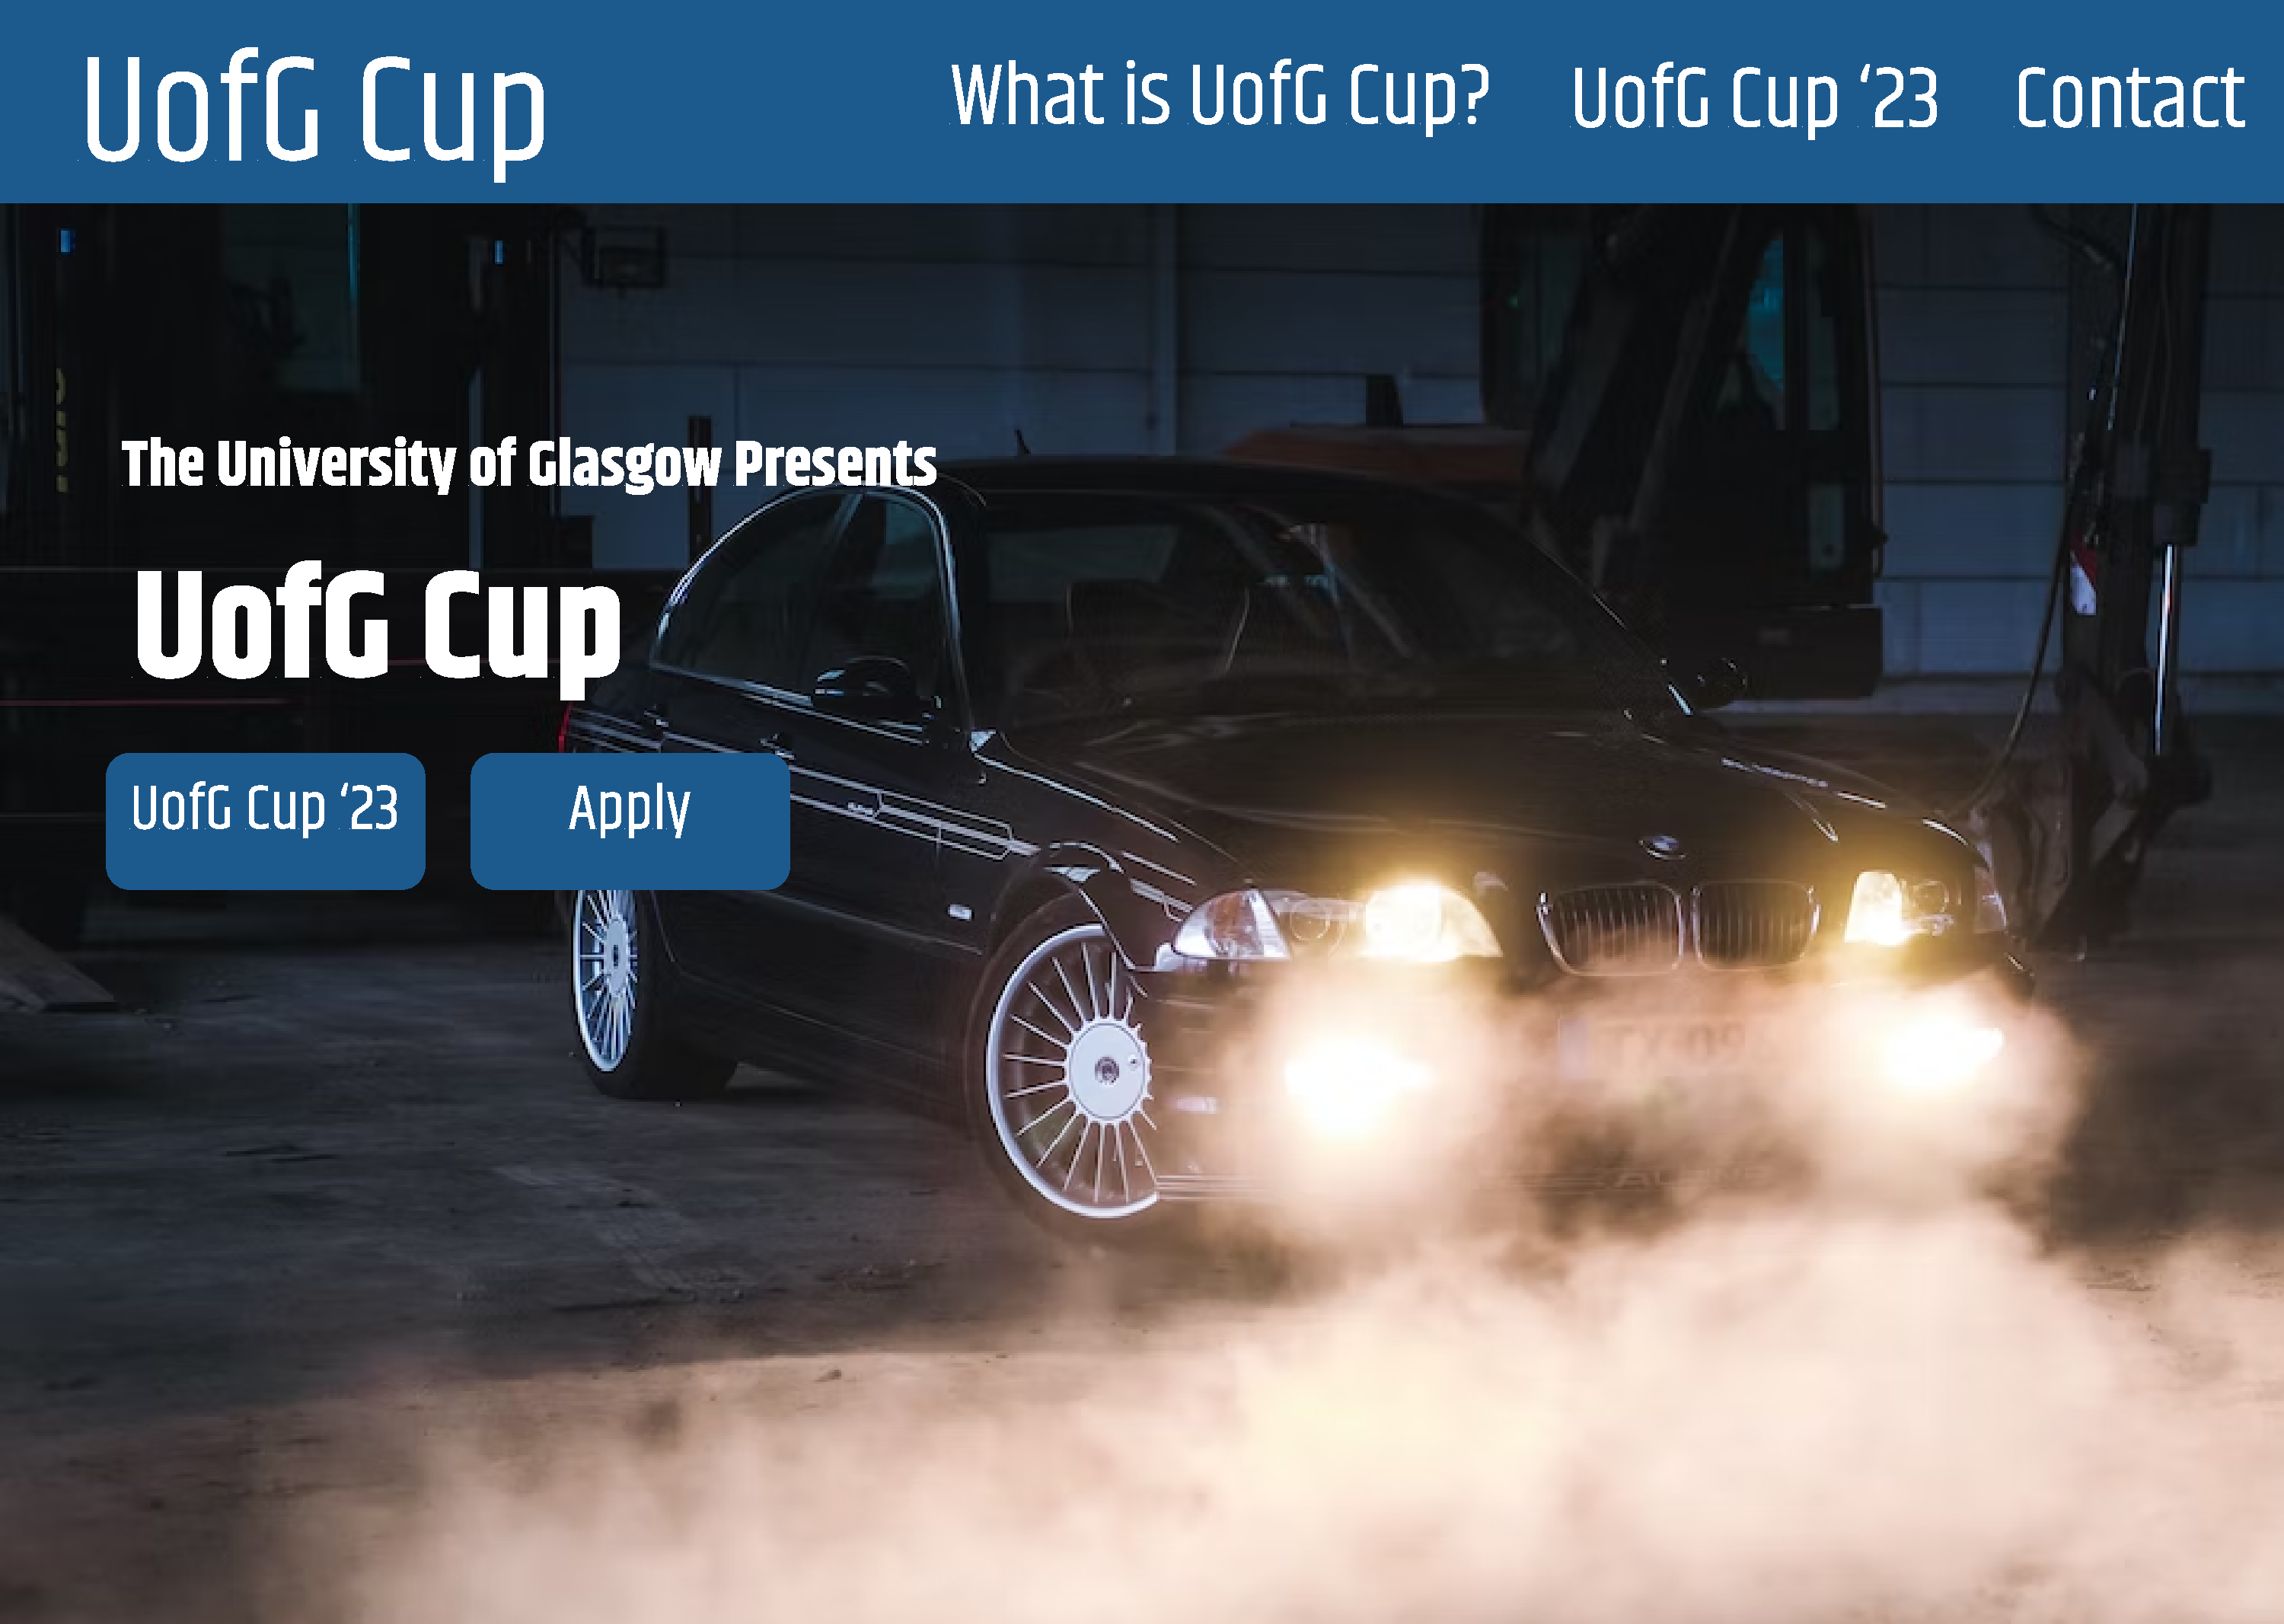
\includegraphics[width=\textwidth]{images/Home.pdf}
        \caption{Home page.}
        \label{fig:web-home-page}  
    \end{subfigure}
    \begin{subfigure}{0.49\textwidth}
        \centering
        \includegraphics[width=\textwidth]{images/What is UofG Cup_.pdf}
        \caption{General Description page.}
        \label{fig:web-gen-desc-page}  
    \end{subfigure}
    
    \begin{subfigure}{0.49\textwidth}
        \centering
        \includegraphics[width=\textwidth]{images/UofG Cup '23.pdf}
        \caption{Competition Description page.}
        \label{fig:web-comp-desc-page}  
    \end{subfigure}
    \begin{subfigure}{0.49\textwidth}
        \centering
        \includegraphics[width=\textwidth]{images/Apply.pdf}
        \caption{Apply page.}
        \label{fig:web-apply-page}  
    \end{subfigure}

    \begin{subfigure}{0.49\textwidth}
        \centering
        \includegraphics[width=\textwidth]{images/User.pdf}
        \caption{User page.}
        \label{fig:web-user-page}  
    \end{subfigure}
    \begin{subfigure}{0.49\textwidth}
        \centering
        \includegraphics[width=\textwidth]{images/Past Competitions.pdf}
        \caption{Past Competitions page.}
        \label{fig:web-past-page}  
    \end{subfigure}
    
    \caption{Figures show various wireframes developed for the robot competition. These wireframes use the name \textit{'UofG Cup'} to refer to the competition.}
    \label{fig:website-wireframes}
\end{figure}



\chapter{Controller Design}\label{sec:controller-design-appendix}

\begin{figure}[!ht]
    \centering
    \includegraphics[width=0.85\linewidth]{images/nintendo-controller.jpg}
    \caption{The Super Nintendo controller. This is designed to be held with two hands with the users thumbs operating the controller. The left thumb controls the directional-pad, and the right thumb controls the functional buttons. The joystick designed for this project takes inspiration from this design.}
    \label{fig:nintendo-controller}
\end{figure}

\begin{figure}[!ht]
    \centering
    \includegraphics[width=0.6\linewidth]{images/buffer.pdf}
    \caption{A diagram of how the queue buffer mechanism works. The first step shows how pairs of motor speeds are added to the buffer. Then, every $x$ seconds, a pair of motor speeds is removed from the front of the buffer and sent to the robot.}
    \label{fig:buffer}
\end{figure}

\begin{figure}[!ht]
    \centering
    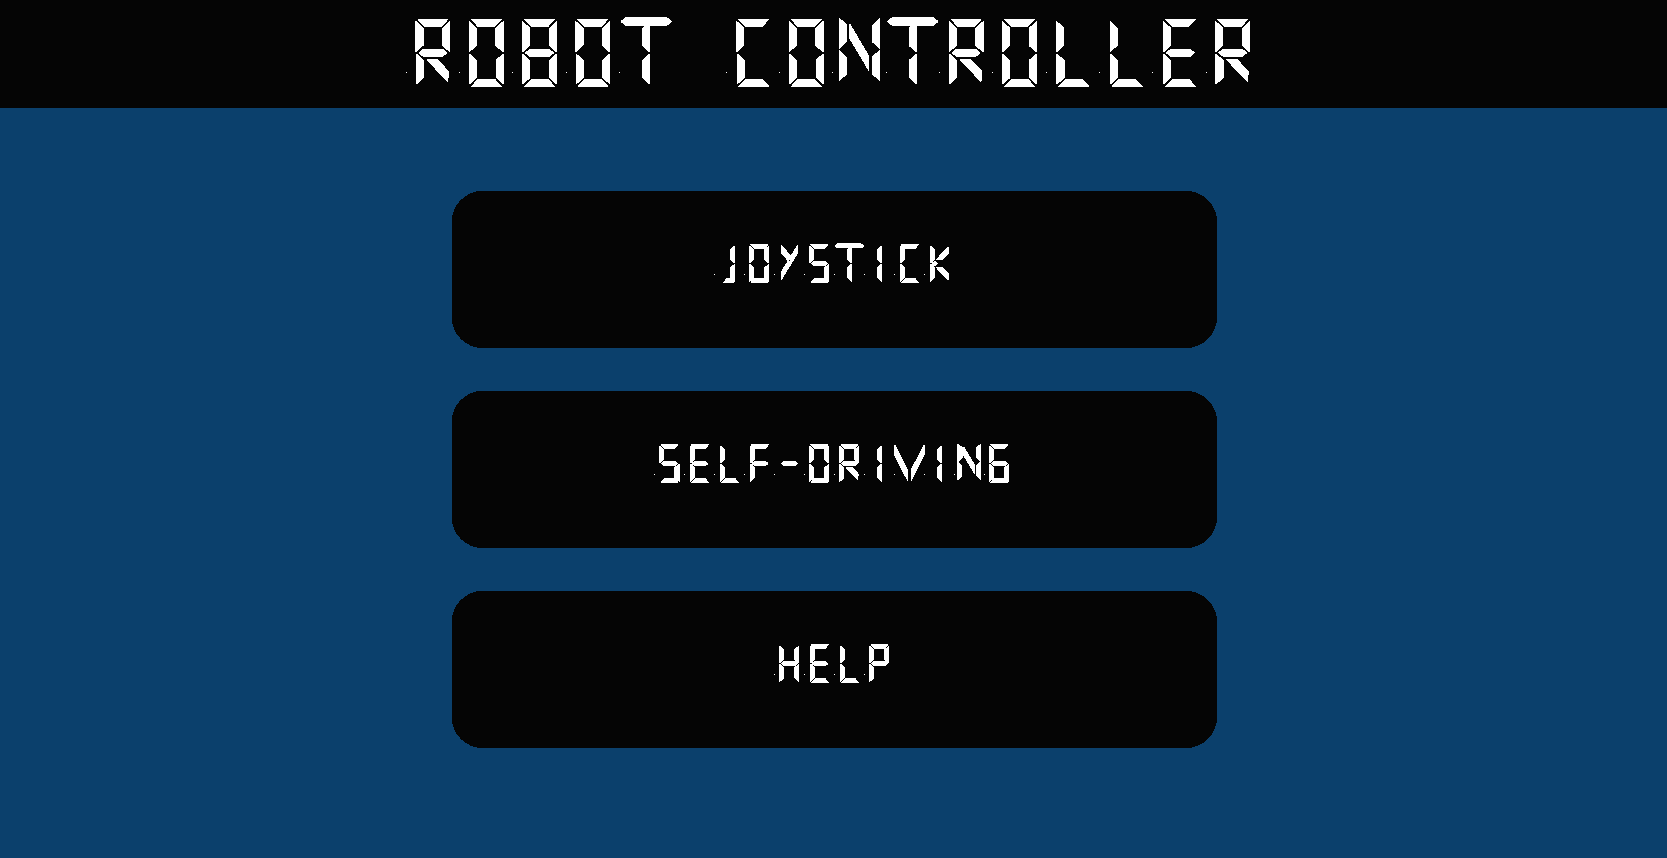
\includegraphics[width=0.7\textwidth]{images/home-page-wireframe.pdf}
    \caption{Wireframe design for Home page.}
    \label{fig:home-page-wireframe} 
\end{figure}

\begin{figure}[!ht]
    \centering
    \begin{subfigure}{0.67\textwidth}
        \centering
        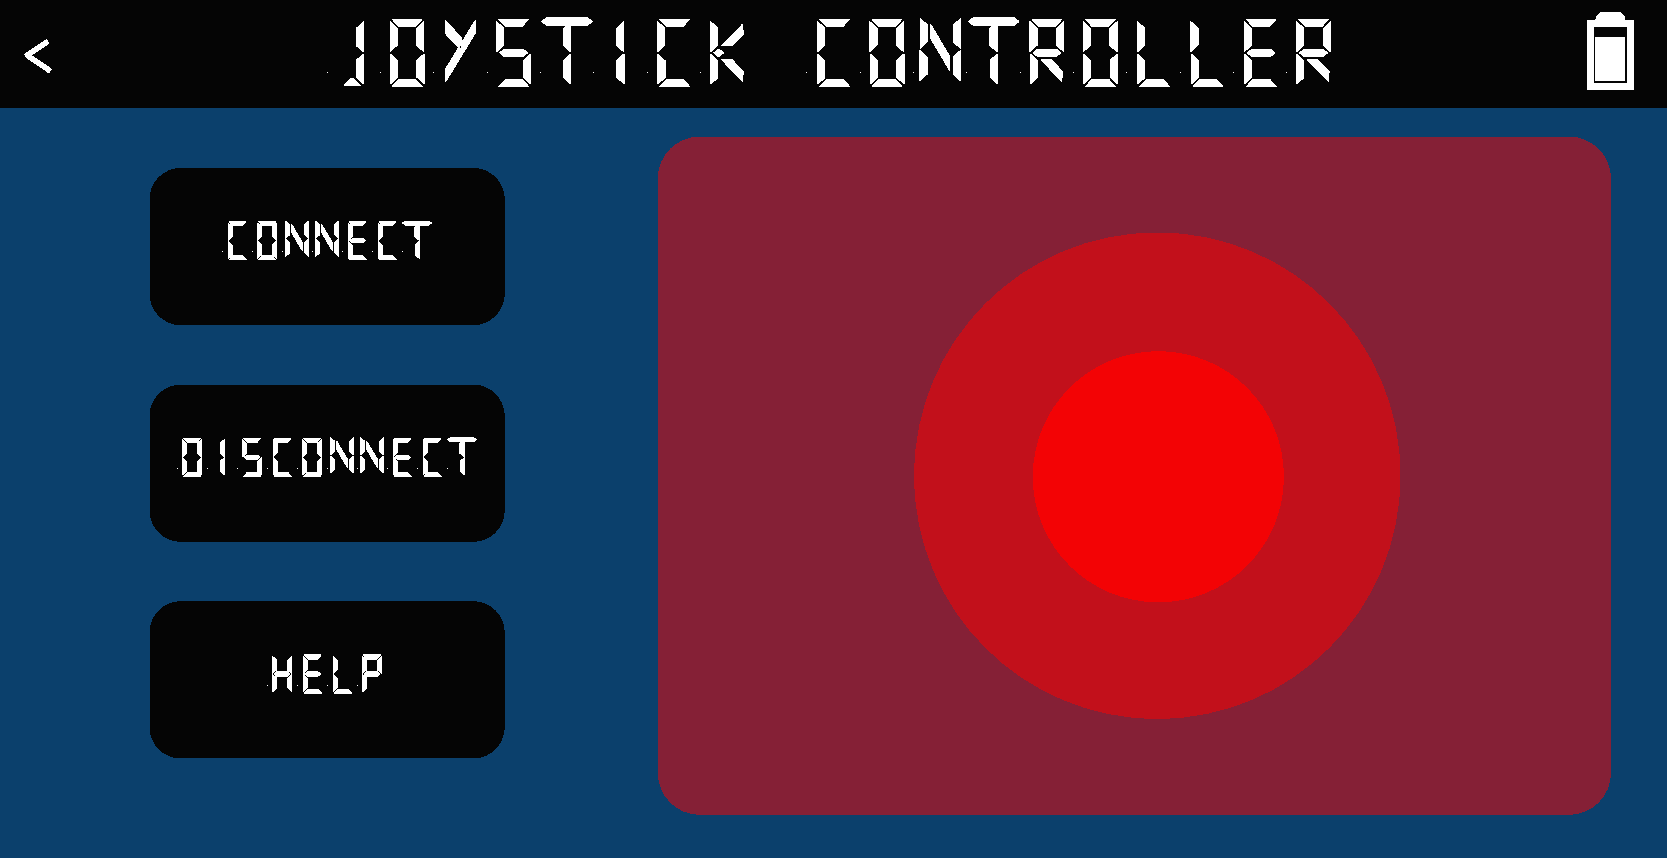
\includegraphics[width=\textwidth]{images/joystick-wireframe.pdf}
        \caption{Landscape.}
        \label{fig:joystick-wireframe} 
    \end{subfigure}
    \begin{subfigure}{0.32\textwidth}
        \centering
        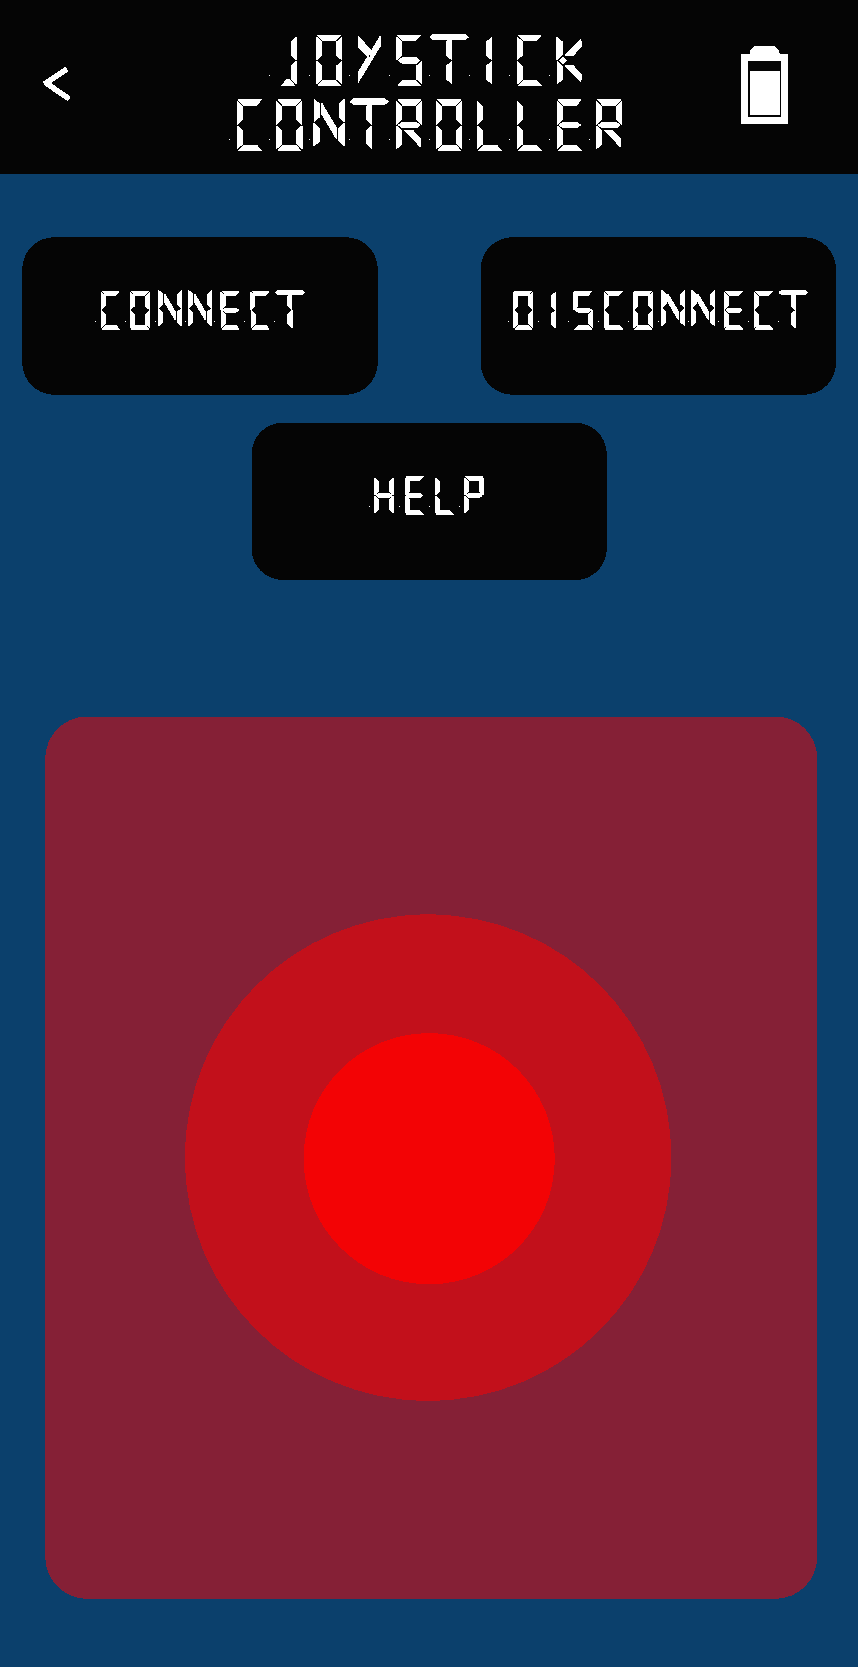
\includegraphics[width=\textwidth]{images/joystick-wireframe-2.pdf}
        \caption{Portrait.}
        \label{fig:joystick-wireframe-2} 
    \end{subfigure}
    \caption{Wireframe designs for Joystick page.}
\end{figure}

\begin{figure}[!h]
    \centering
    \begin{subfigure}{0.67\textwidth}
        \centering
        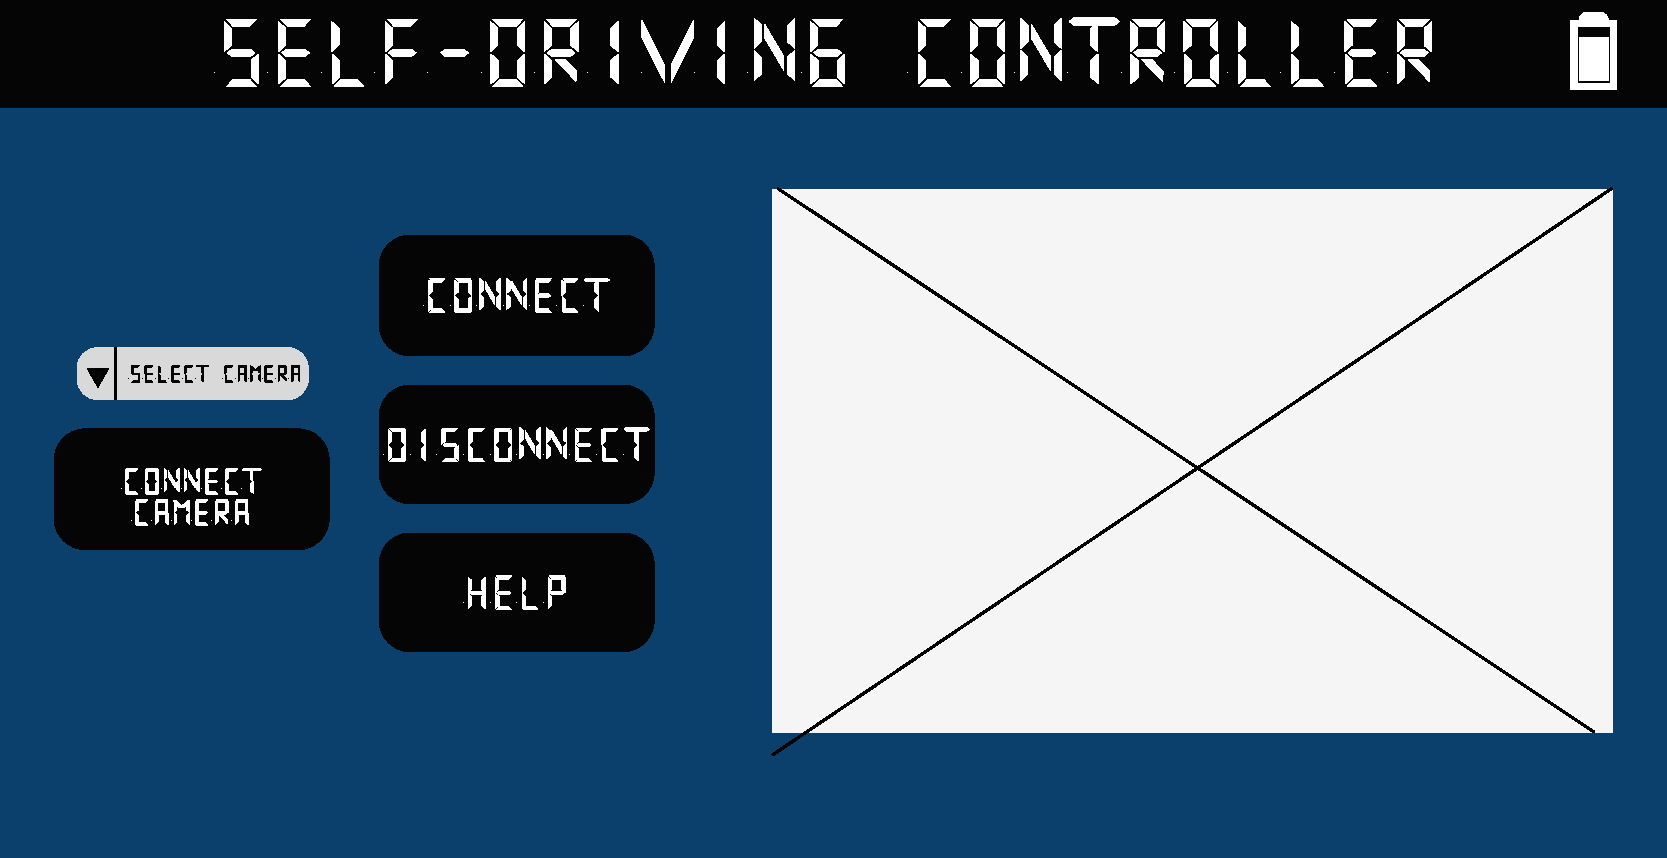
\includegraphics[width=\textwidth]{images/host-wireframe.pdf}
        \caption{Wireframe design for Self-Driving page.}
        \label{fig:host-wireframe} 
    \end{subfigure}
    \begin{subfigure}{0.32\textwidth}
        \centering
        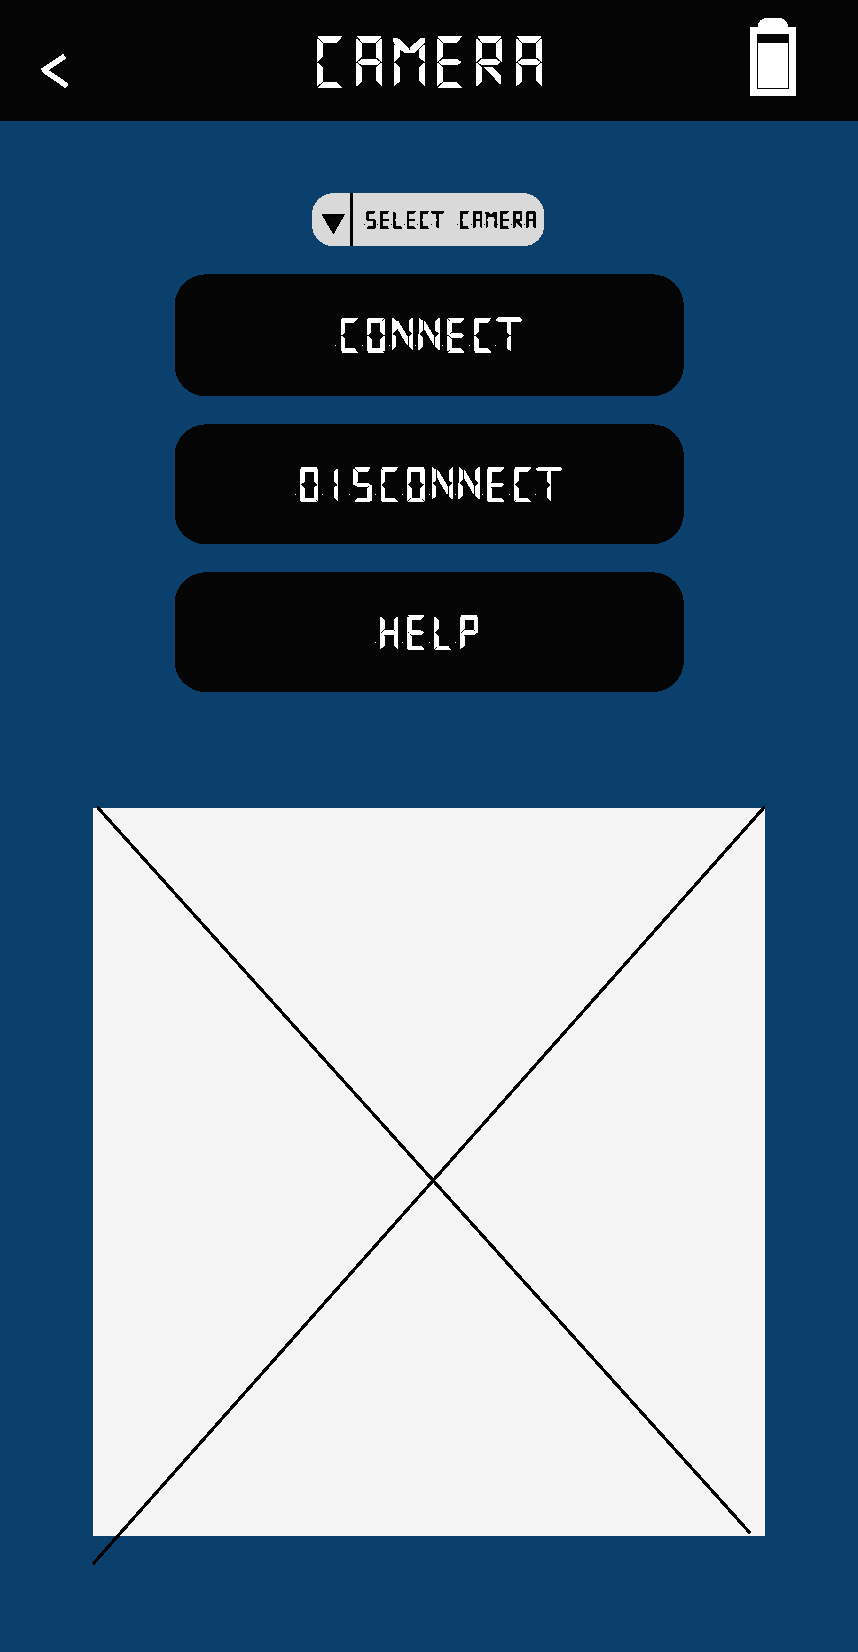
\includegraphics[width=\textwidth]{images/peer-wireframe.pdf}
        \caption{Wireframe design for Peer page.}
        \label{fig:peer-wireframe} 
    \end{subfigure}
    \caption{Wireframe designs for self-driving and peer page.}
    \label{fig:controller-wireframes}
\end{figure}


\chapter{Controller Code}
\begin{figure}[!h]
    \centering
    \begin{subfigure}{0.49\textwidth}
        \begin{lstlisting}
        connectRobot = (): void => {
          UART.connect((c: any) => {
            if (!c || null) {
              console.log("not connected");
            } else {
              connection = c;
              isConnected = true;
            }
          });
        };
        \end{lstlisting}
    \caption{Connect function for connecting to robot.}
    \label{lst:connect-func}
    \end{subfigure}
    \begin{subfigure}{0.49\textwidth}
        \begin{lstlisting}
        disconnectRobot = (): void => {
          UART.close();
          this.isConnected = false;
        };
        \end{lstlisting}
    \caption{Disconnect function for disconnecting to robot.}
    \label{lst:disconnect-func}
    \end{subfigure}
    \caption{Functions for connecting and disconnecting from the robot. \subref{lst:connect-func} shows the connect function establishing a UART connection with the Pixl.js. \subref{lst:disconnect-func} shows the UART connection being closed.}
    \label{lst:connection-funcs}
\end{figure}


\begin{figure}[!h]
    \centering
        \begin{lstlisting}
        sendCode(): void {
          const speed = this.#buffer.pop();
          if (speed) {
            connection.write(`move(${speed[0]},${speed[1]});\n`);
          };
        };
        \end{lstlisting}
    \caption{Figure shows the \lstinline{sendCode()} function, which removes a speed from the buffer and sends it to the robot via the UART connection.}
    \label{lst:send-code}
\end{figure}


\begin{figure}[!h]
    \centering
        \begin{lstlisting}
        var Piecewise = require('piecewise-function');

        export class AngleMotorMapping {
          name: string;
          angles: any;
          leftMotorMapping: any;
          rightMotorMapping: any;
        
          constructor(name: string, angles: any, leftMotorMapping: any, rightMotorMapping: any) {
            this.name = name;
            this.angles = angles;
            this.leftMotorMapping = Piecewise(angles, leftMotorMapping);
            this.rightMotorMapping = Piecewise(angles, rightMotorMapping);
          };
        };
        const tightControl = new AngleMotorMapping("Tight Control",
          [0, 45, 90, 135, 180, 225, 225.1, 270, 314.9, 315, 360],
          [1, 1, 1, 0, 0, 0, 0, -1, -1, 1, 1],
          [0, 0, 1, 1, 1, 1, -1, -1, 0, 0, 0]
        );
        const looseControl = new AngleMotorMapping("Loose Control",
          [0, 45, 90, 135, 180, 180.1, 225, 270, 315, 359.9, 360],
          [1, 1, 1, 0.5, 0, 0, -0.5, -1, -1, -1, 1],
          [0, 0.5, 1, 1, 1, -1, -1, -1, -0.5, 0, 0]
        );
        \end{lstlisting}
    \caption{The AngleMotorMapping class. This creates a piecewise function for both the left and right motors, using their pre-set values at specific angles.}
    \label{lst:angleMotorMappings}
\end{figure}

\begin{figure}[!h]
    \begin{lstlisting}
    const getOrientationVector = (c1, c2): {x: number, y: number} => {
      const dx = c2.x - c1.x;
      const dy = c2.y - c1.y;
      const orientation =  Math.atan2(dy, dx);
      return { x: Math.cos(orientation), y: Math.sin(orientation) };
    };
    \end{lstlisting}
\caption{\lstinline{getOrientationVector()} calculates orientation of a marker.}
\label{lst:orientation-code}
\end{figure}

\begin{figure}[!h]
    \begin{lstlisting}
    const getDirectionVector = (c1, c2): {x: number, y: number} => {
      const x = (c1.x + c2.x)/2
      const y = (c1.y + c2.y)/2
      const dx = canvasMidpoint.x - x;
      const dy = canvasMidpoint.y - y;
      return { x: dx, y: dy };
    };
    \end{lstlisting}
\caption{\lstinline{getDirectionVector()} calculates direction of a marker with respect to the mid-point of the camera.}
\label{lst:direction-code}
\end{figure}

\begin{figure}
    \centering
    \includegraphics[width=1\textwidth]{images/code-editor-nocode.png}
    \caption{Screenshot shows the code check on the controller. On the right half we see there is currently no code on the robot. By selecting "upload code", we can upload the code on the left half to the robot.}
    \label{fig:code-editor}
\end{figure}



\chapter{Evaluation: Questionnaire Results}

\begin{table}[!ht]
\centering
\caption{Table shows the number of collisions that occurred for each participant. The best column shows the trial where the participant collided with the least amount of obstacles. Finally, the table also shows the total number of obstacles collided with per task, and the total number of participants who collided with an obstacle during their trial.}
\label{tab:joystick-collisions}
\begin{tabular}{ccccccc}
\textbf{Task} & \multicolumn{3}{c}{Single Obstacle} & \multicolumn{3}{c}{Slalom} \\
\textbf{Mapping} & Tight & Loose & Best & Tight & Loose & Best \\
User 1 & 0 & 0 & 0 & 0 & 0 & 0 \\
User 2 & 1 & 0 & 0 & 2 & 2 & 2 \\
User 3 & 0 & 0 & 0 & 0 & 1 & 0 \\
User 4 & 0 & 0 & 0 & 1 & 0 & 0 \\
User 5 & 0 & 0 & 0 & 0 & 0 & 0 \\
User 6 & 1 & 0 & 0 & 1 & 0 & 0 \\
User 7 & 0 & 0 & 0 & 0 & 0 & 0 \\
User 8 & 0 & 0 & 0 & 0 & 2 & 0 \\
User 9 & 0 & 0 & 0 & 0 & 0 & 0 \\
User 10 & 0 & 0 & 0 & 0 & 1 & 0 \\
\textbf{Total Obstacles} & \textbf{2} & \textbf{0} & \textbf{0} & \textbf{4} & \textbf{6} & \textbf{2} \\
\textbf{Total Participants} & \textbf{2} & \textbf{0} & \textbf{0} & \textbf{3} & \textbf{4} & \textbf{1}
\end{tabular}
\end{table}

\begin{table}[!ht]
\centering
\caption{Tables shows the time taken for participants to navigate the robot through the given tasks. The best column, shows the faster time between the trials for the tight and loose mappings. The table also shows the average time taken.}
\label{tab:joystick-times}
\begin{tabular}{ccccccc}
\textbf{Task} & \multicolumn{3}{c}{Single Obstacle} & \multicolumn{3}{c}{Slalom} \\
\textbf{Mapping} & Tight & Loose & Best & Tight & Loose & Best \\
User 1 & 10.34 & 10.89 & 10.34 & 35.23 & 39.98 & 35.23 \\
User 2 & 13.8 & 8.52 & 8.52 & 52.52 & 58.12 & 52.52 \\
User 3 & 12.82 & 13.1 & 12.82 & 38.84 & 40.12 & 38.84 \\
User 4 & 14.72 & 10.18 & 10.18 & 50.23 & 47.45 & 47.45 \\
User 5 & 11.32 & 10.11 & 10.11 & 41.51 & 45.78 & 41.51 \\
User 6 & 13.03 & 11.86 & 11.86 & 39.87 & 43.99 & 39.87 \\
User 7 & 10.94 & 13.89 & 10.94 & 41.67 & 53.22 & 41.67 \\
User 8 & 11.92 & 13.32 & 11.92 & 40.73 & 53.61 & 40.73 \\
User 9 & 10.76 & 12.31 & 10.76 & 51.45 & 42.76 & 42.76 \\
User 10 & 10.57 & 12.21 & 10.57 & 38.98 & 47.12 & 38.98 \\
\textbf{Average Time} & \textbf{12.022} & \textbf{11.639} & \textbf{10.802} & \textbf{43.103} & \textbf{47.215} & \textbf{41.956}
\end{tabular}
\end{table}

\begin{figure}
    \centering
    \includegraphics[width=0.9\textwidth]{images/responsive-joystick-results.png}
    \caption{Bar graph showing the results obtained for the question "How responsive did you find the joystick to use?". In this question, 1 correlates to "Not very responsive" and 10 correlates to "very responsive". These results give an average score of 9.5.}
    \label{fig:joystick-responsive-results}
\end{figure}

\\\\

\begin{figure}[!ht]
    \centering
    \begin{subfigure}{0.9\textwidth}
        \includegraphics[width=\textwidth]{images/joystick-object-difficulty.png}
        \label{fig:joystick-object-difficulty}
        \caption{The results when asked about the difficulty of navigating around the object using the joystick.}
    \end{subfigure}
    \begin{subfigure}{0.9\textwidth}
        \includegraphics[width=\textwidth]{images/joystick-slalom-difficulty.png}
        \label{fig:joystick-slalom-difficulty}
        \caption{The results when asked about the difficulty of navigating through the slalom using the joystick.}
    \end{subfigure}
    \caption{Bar graph showing the results for questions obtained from the questionnaire. Figure \subref{fig:joystick-object-difficulty} shows the results when asked about the difficulty of navigating the robot using the joystick around an object, while Figure \subref{fig:joystick-slalom-difficulty} shows the results when asked about the difficulty of going through the slalom with the joystick. A score of 1 correlates to "very easy", while a score of 10 correlates to "very difficult".}
    \label{fig:manual-difficulty}
\end{figure}


\begin{figure}
    \centering
    \includegraphics[width=0.7\textwidth]{images/mapping-preference.png}
    \caption{Pie chart which shows the results when asked which angle motor mapping participants preferred. As seen, there was an equal number of votes between the mappings.}
    \label{fig:mapping-preference}
\end{figure}

\begin{figure}
    \centering
    \includegraphics[width=0.9\textwidth]{images/virtual-lead-responsive.png}
    \caption{Bar graph showing the results obtained for the question "How responsive did you find the Virtual Lead feature to use?". In this question, 1 correlates to "Not very responsive" and 10 correlates to "very responsive". These results give an average score of 3.1.}
    \label{fig:virtual-lead-responsive}
\end{figure}

\begin{figure}
    \centering
    \includegraphics[width=0.9\textwidth]{images/virtual-lead-intuition.png}
    \caption{Bar graph showing the results obtained when asked about how intuitive Virtual Lead was to set-up.}
    \label{fig:virtual-lead-intuition}
\end{figure}

\begin{figure}
    \centering
    \includegraphics[width=1\textwidth]{images/website-questions.pdf}
    \caption{This figure shows feedback from the questionnaire, regarding people's understanding of what the competition is, based off what they read from the website.}
    \label{fig:feedback-1}
\end{figure}

\begin{figure}
    \centering
    \includegraphics[width=1\textwidth]{images/website-question-2.pdf}
    \caption{This figure shows feedback from the questionnaire, regarding if the competition rules were easy to find on the website, and if people would be interested in entering the competition.}
    \label{fig:feedback-2}
\end{figure}


\chapter{Guidance}
Typical inclusions in the appendices are:
\begin{itemize}
\item
  Copies of ethics approvals (required if obtained)
\item
  Copies of questionnaires etc. used to gather data from subjects.
\item
  Extensive tables or figures that are too bulky to fit in the main body of
  the report, particularly ones that are repetitive and summarised in the body.
\item Outline of the source code (e.g. directory structure), or other architecture documentation like class diagrams.
\item User manuals, and any guides to starting/running the software.
\end{itemize}

\end{appendices}

%==================================================================================================================================
%   BIBLIOGRAPHY   

% The bibliography style is abbrvnat
% The bibliography always appears last, after the appendices.

\bibliographystyle{abbrvnat}
\bibliography{l4proj}

\end{document}
